\PassOptionsToPackage{table}{xcolor}
\documentclass[10pt,aspectratio=169]{beamer}

\usetheme{metropolis}
\usepackage{appendixnumberbeamer}
\usepackage{booktabs}
\usepackage{array}
\usepackage{multirow}
\usepackage{tikz}
\usetikzlibrary{
  positioning,
  arrows.meta,
  decorations.pathmorphing,
  calc,
  fit,
  shapes.geometric,
  backgrounds,
  chains,
  matrix,
  decorations.pathreplacing
}
\usepackage{amsmath,amssymb}
\usepackage{xcolor}

% --- Colors ---
\definecolor{accent}{HTML}{3498DB}
\definecolor{phoneme}{HTML}{E74C3C}
\definecolor{circuit}{HTML}{27AE60}
\definecolor{backbone}{HTML}{F39C12}
\definecolor{fusion}{HTML}{9B59B6}
\definecolor{chill}{HTML}{95A5A6}
\definecolor{tok}{HTML}{E67E22}

\setbeamercolor{alerted text}{fg=phoneme}

\hypersetup{
  colorlinks=true,
  linkcolor=black,
  urlcolor=accent,
  citecolor=accent
}

\title{Phonological Assembly Circuits in GPT-2}
\subtitle{How Transformers Compute Sound Structure from Orthography}
\author{Elliot Tower}
\date{}

\begin{document}

% =============================================
% TITLE
% =============================================
\begin{frame}[plain]
\maketitle
\end{frame}

% =============================================
% OVERVIEW
% =============================================
\begin{frame}{Overview}
\hypertarget{sl:overview}{}

\begin{columns}[T]
\begin{column}{0.31\textwidth}
\textbf{\hyperlink{sl:motivation}{Part 1: The Question}}
\begin{enumerate}
  \item \hyperlink{sl:motivation}{Motivation}
  \item \hyperlink{sl:operations}{Six operations}
  \item \hyperlink{sl:oronym}{Chained operations}
\end{enumerate}

\vspace{0.6em}
\textbf{\hyperlink{sl:datasets}{Part 2: Methods}}
\begin{enumerate}\setcounter{enumi}{3}
  \item \hyperlink{sl:datasets}{Datasets}
  \item \hyperlink{sl:discovery}{Analysis pipeline}
\end{enumerate}

\vspace{0.6em}
\textbf{\hyperlink{sl:backbone}{Part 3: Hypotheses}}
\begin{enumerate}\setcounter{enumi}{5}
  \item \hyperlink{sl:backbone}{Prior circuits}
  \item \hyperlink{sl:fusionheads}{Three hypotheses}
  \item \hyperlink{sl:composition}{Predictions}
\end{enumerate}
\end{column}

\begin{column}{0.31\textwidth}
\textbf{\hyperlink{sl:results}{Part 4: Circuit Localization}}
\begin{enumerate}\setcounter{enumi}{8}
  \item \hyperlink{sl:behavioral}{Behavioral validation}
  \item \hyperlink{sl:eapresults}{EAP-IG circuits}
\end{enumerate}

\vspace{0.6em}
\textbf{\hyperlink{sl:validation}{Part 5: Circuit Validation}}
\begin{enumerate}\setcounter{enumi}{10}
  \item \hyperlink{sl:circuitoverlap}{Cross-task overlap}
  \item Compositional reuse
  \item \hyperlink{sl:causaldiscovery}{Causal inference}
\end{enumerate}

\vspace{0.6em}
\textbf{\hyperlink{sl:cvl}{Part 6: Causal Variable Localization}}
\begin{enumerate}\setcounter{enumi}{13}
  \item \hyperlink{sl:cvl}{What flows along edges?}
  \item \hyperlink{sl:dasresults}{DAS results}
\end{enumerate}
\end{column}

\begin{column}{0.31\textwidth}
\textbf{\hyperlink{sl:discussion}{Part 7: Implications}}
\begin{enumerate}\setcounter{enumi}{15}
  \item \hyperlink{sl:discussion}{Causal abstraction}
  \item \hyperlink{sl:mechanism}{What is a mechanism?}
  \item \hyperlink{sl:cogsci}{Cognitive science parallel}
  \item \hyperlink{sl:tooling}{Limitations}
  \item Future: causal graph discovery
\end{enumerate}
\end{column}
\end{columns}
\end{frame}

% =============================================
% PART 1 DIVIDER
% =============================================
\begin{frame}[plain,noframenumbering]
\begin{center}
\vfill
  {\setlength{\fboxrule}{2.5pt}\fcolorbox{black}{white}{\parbox{0.7\textwidth}{\centering\vspace{0.8em}
    {\Large\bfseries Part 1: The Question}
  \vspace{0.8em}}}}
\vfill
\end{center}
\end{frame}

% =============================================
% MOTIVATION
% =============================================
\begin{frame}{Why phonological circuits?}
\hypertarget{sl:motivation}{}

The MI literature has characterized circuits for:
\begin{itemize}
  \item Syntax: \href{https://arxiv.org/abs/2211.00593}{IOI} (Wang et al., 2023), subject--verb agreement, reflexive anaphora
  \item Retrieval: induction heads, greater-than
  \item Factual: capital cities, birth years
\end{itemize}

\vspace{0.8em}
\textbf{Gap:} zero circuit-level work on \alert{phonological} computation.

\vspace{0.8em}
Yet LLMs demonstrably encode sound structure:
\begin{itemize}
  \item Linear probes on GPT-2 mid-layers: 63--79\% rhyme detection (\href{https://aclanthology.org/2026.latechclfl-1.9}{Liao \& Shi, 2026})
  \item Above-chance grapheme-to-phoneme conversion (\href{https://arxiv.org/abs/2404.02456}{PhonologyBench, 2024})
\end{itemize}

\vspace{0.8em}
\textbf{Question:} \emph{Which attention heads compute phonological knowledge?}
\end{frame}

% =============================================
% THE PUZZLE
% =============================================
\begin{frame}{The puzzle}

BPE tokenization encodes \textbf{orthography}, not phonology.

\vspace{0.5em}
Yet the model can do this:

\vspace{0.8em}
\begin{center}
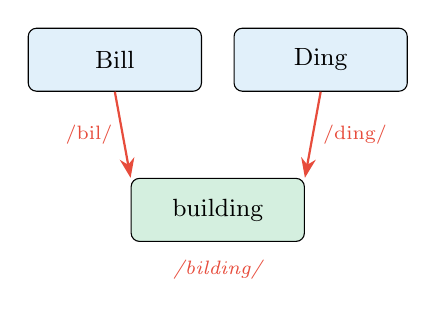
\begin{tikzpicture}[
  box/.style={draw, rounded corners=3pt, minimum height=0.8cm, minimum width=2.2cm, font=\small},
  arr/.style={-{Stealth[length=2.5mm]}, thick}
]
  \node[box, fill=accent!15] (bill) {Bill};
  \node[box, fill=accent!15, right=0.4cm of bill] (ding) {Ding};

  \node[box, fill=circuit!20, below=1.5cm of $(bill)!0.5!(ding)$] (building) {building};

  \draw[arr, phoneme] (bill.south) -- (building.north west) node[midway, left, font=\scriptsize] {/bil/};
  \draw[arr, phoneme] (ding.south) -- (building.north east) node[midway, right, font=\scriptsize] {/ding/};
  \node[below=0.1cm of building, font=\scriptsize\itshape, phoneme] {/bilding/};
\end{tikzpicture}
\end{center}

\vspace{0.5em}
\textbf{Cross-boundary phoneme fusion} from purely orthographic input.

How? Which heads? Is there a dedicated circuit?
\end{frame}

% =============================================
% THE SIX OPERATIONS
% =============================================
\begin{frame}{Six phonological operations}
\hypertarget{sl:operations}{}

\begin{center}
\small
\begin{tabular}{clllr}
\toprule
\textbf{Op} & \textbf{Linguistic term} & \textbf{Example} & \textbf{Computation} & \textbf{N} \\
\midrule
1 & Rhyming hypocorism & Robert $\to$ Bob & Irregular stored lookup & 32 \\
2 & Clipping (apocope) & Timothy $\to$ Tim & First-syllable truncation & 90 \\
3 & Initialism & J $\to$ Jay & Grapheme $\to$ phoneme name & 30 \\
4 & \textbf{Oronym} & \textbf{Bill Ding $\to$ building} & \textbf{Cross-boundary fusion} & \textbf{99} \\
5 & Homophone & Neil $\to$ kneel & Phoneme-identity detection & 120 \\
6 & Folk etymology & curtain $\to$ Curt & Reverse decomposition & 75 \\
\bottomrule
\end{tabular}
\end{center}

\vspace{0.5em}
Each requires a \textbf{linguistically distinct} computation.

$\to$ Predicts \textbf{distinct circuit architectures}.
\end{frame}

% =============================================
% OPERATIONS DIAGRAM
% =============================================
\begin{frame}{Operations as a computational taxonomy}

\begin{center}
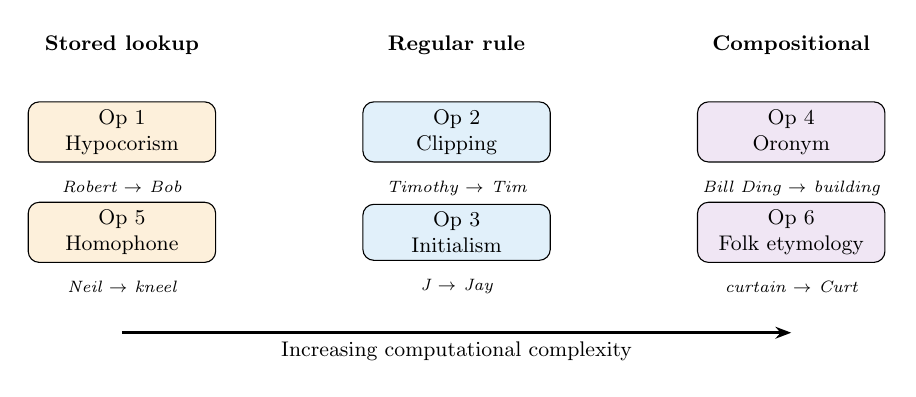
\begin{tikzpicture}[
  scale=0.85, transform shape,
  op/.style={draw, rounded corners=4pt, minimum height=0.7cm, minimum width=2.8cm,
             font=\small, align=center},
  cat/.style={draw=none, font=\small\bfseries, text=black},
  arr/.style={-{Stealth[length=2mm]}, thick, black}
]
  % Categories
  \node[cat] (stored) at (0, 2.5) {Stored lookup};
  \node[cat] (regular) at (5, 2.5) {Regular rule};
  \node[cat] (compositional) at (10, 2.5) {Compositional};

  % Operations
  \node[op, fill=backbone!15] (op1) at (0, 1.2) {Op 1\\Hypocorism};
  \node[op, fill=backbone!15] (op5) at (0, -0.3) {Op 5\\Homophone};

  \node[op, fill=accent!15] (op2) at (5, 1.2) {Op 2\\Clipping};
  \node[op, fill=accent!15] (op3) at (5, -0.3) {Op 3\\Initialism};

  \node[op, fill=fusion!15] (op4) at (10, 1.2) {Op 4\\Oronym};
  \node[op, fill=fusion!15] (op6) at (10, -0.3) {Op 6\\Folk etymology};

  % Examples
  \node[font=\scriptsize\itshape, below=0.15cm of op1] {Robert $\to$ Bob};
  \node[font=\scriptsize\itshape, below=0.15cm of op5] {Neil $\to$ kneel};
  \node[font=\scriptsize\itshape, below=0.15cm of op2] {Timothy $\to$ Tim};
  \node[font=\scriptsize\itshape, below=0.15cm of op3] {J $\to$ Jay};
  \node[font=\scriptsize\itshape, below=0.15cm of op4] {Bill Ding $\to$ building};
  \node[font=\scriptsize\itshape, below=0.15cm of op6] {curtain $\to$ Curt};

  % Difficulty arrow
  \draw[arr, very thick, black] (0, -1.8) -- (10, -1.8)
    node[midway, below, font=\small] {Increasing computational complexity};
\end{tikzpicture}
\end{center}

\vspace{0.3em}
Stored $\to$ Regular $\to$ Compositional: each category demands more computation.

Op 4 (oronym) requires \textbf{cross-token phoneme assembly} --- the hardest operation.
\end{frame}

% =============================================
% THE ORONYM PROBLEM
% =============================================
\begin{frame}{The oronym problem}
\hypertarget{sl:oronym}{}

\begin{center}
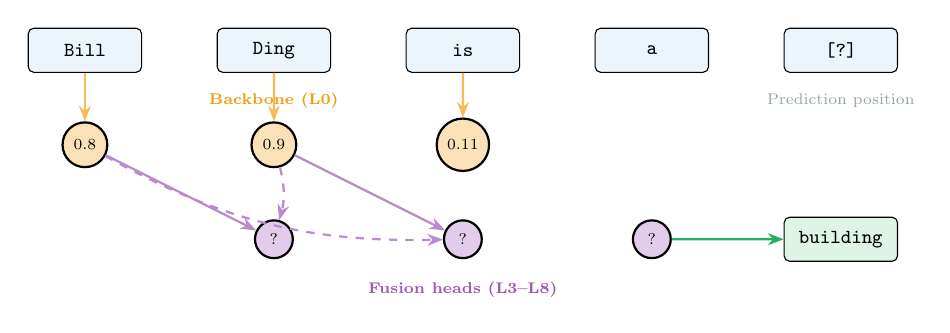
\begin{tikzpicture}[
  scale=0.8, transform shape,
  token/.style={draw, rounded corners=2pt, minimum height=0.7cm, font=\small,
                fill=accent!10, minimum width=1.8cm},
  head/.style={circle, draw, minimum size=0.6cm, font=\scriptsize, thick},
  arr/.style={-{Stealth[length=2mm]}, thick}
]
  % Input tokens
  \node[token] (t1) at (0, 4) {\texttt{Bill}};
  \node[token] (t2) at (3, 4) {\texttt{Ding}};
  \node[token] (t3) at (6, 4) {\texttt{is}};
  \node[token] (t4) at (9, 4) {\texttt{a}};
  \node[token] (t5) at (12, 4) {\texttt{[?]}};

  % Layer 0 - backbone
  \node[head, fill=backbone!30] (h08) at (0, 2.5) {0.8};
  \node[head, fill=backbone!30] (h09) at (3, 2.5) {0.9};
  \node[head, fill=backbone!30] (h011) at (6, 2.5) {0.11};

  % Mid-layer - fusion
  \node[head, fill=fusion!30] (hf1) at (3, 1) {?};
  \node[head, fill=fusion!30] (hf2) at (6, 1) {?};
  \node[head, fill=fusion!30] (hf3) at (9, 1) {?};
  \node[font=\scriptsize\bfseries, fusion] at (6, 0.2) {Fusion heads (L3--L8)};

  % Output
  \node[token, fill=circuit!15] (out) at (12, 1) {\texttt{building}};

  % Connections
  \draw[arr, backbone!70] (t1) -- (h08);
  \draw[arr, backbone!70] (t2) -- (h09);
  \draw[arr, backbone!70] (t3) -- (h011);

  \draw[arr, fusion!70] (h08) -- (hf1);
  \draw[arr, fusion!70] (h09) -- (hf2);
  \draw[arr, fusion!70, dashed] (h08) to[bend right=15] (hf2);
  \draw[arr, fusion!70, dashed] (h09) to[bend left=15] (hf1);

  \draw[arr, circuit] (hf3) -- (out);

  % Labels
  \node[font=\scriptsize\bfseries, backbone] at (3, 3.2) {Backbone (L0)};
  \node[font=\scriptsize, chill] at (12, 3.2) {Prediction position};
\end{tikzpicture}
\end{center}

\vspace{0.3em}
\textbf{Expected:} fusion heads attend \emph{across} the word boundary,\\
composing phonemes from both ``Bill'' and ``Ding'' into ``building.''
\end{frame}

% =============================================
% COMPOUND PUNS
% =============================================
\begin{frame}{Chained operations: shorten + fusion}

\begin{center}
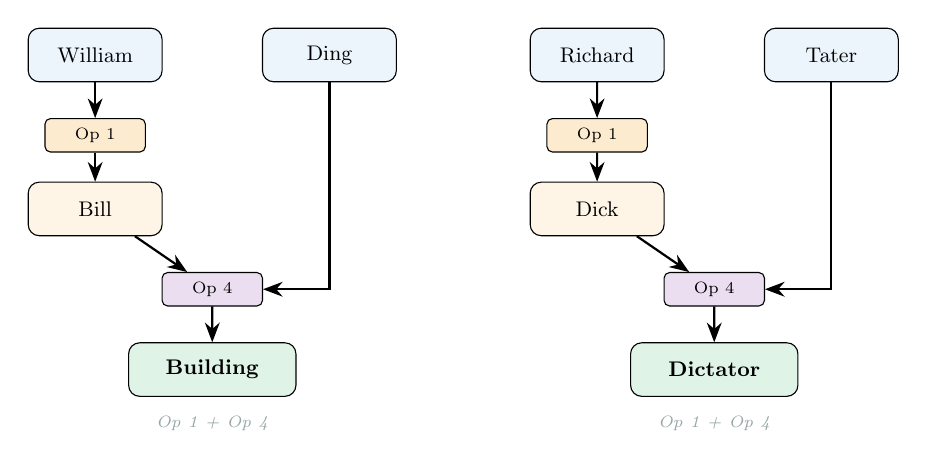
\begin{tikzpicture}[
  scale=0.85, transform shape,
  box/.style={draw, rounded corners=4pt, minimum height=0.8cm, font=\small,
              minimum width=2cm, align=center},
  opbox/.style={draw, rounded corners=2pt, minimum height=0.5cm, font=\scriptsize,
                fill=chill!15, minimum width=1.5cm},
  arr/.style={-{Stealth[length=2.5mm]}, thick}
]
  % William Ding -> Building
  \node[box, fill=accent!10] (william) at (0, 2) {William};
  \node[box, fill=accent!10] (ding) at (3.5, 2) {Ding};

  \node[opbox, fill=backbone!20] (op1a) at (0, 0.8) {Op 1};
  \node[box, fill=backbone!10] (bill) at (0, -0.3) {Bill};

  \node[opbox, fill=fusion!20] (op4a) at (1.75, -1.5) {Op 4};
  \node[box, fill=circuit!15, minimum width=2.5cm] (building) at (1.75, -2.7) {\textbf{Building}};

  \draw[arr] (william) -- (op1a);
  \draw[arr] (op1a) -- (bill);
  \draw[arr] (bill) -- (op4a);
  \draw[arr] (ding) |- (op4a);
  \draw[arr] (op4a) -- (building);

  % Richard Tater -> Dictator
  \node[box, fill=accent!10] (richard) at (7.5, 2) {Richard};
  \node[box, fill=accent!10] (tater) at (11, 2) {Tater};

  \node[opbox, fill=backbone!20] (op1b) at (7.5, 0.8) {Op 1};
  \node[box, fill=backbone!10] (dick) at (7.5, -0.3) {Dick};

  \node[opbox, fill=fusion!20] (op4b) at (9.25, -1.5) {Op 4};
  \node[box, fill=circuit!15, minimum width=2.5cm] (dictator) at (9.25, -2.7) {\textbf{Dictator}};

  \draw[arr] (richard) -- (op1b);
  \draw[arr] (op1b) -- (dick);
  \draw[arr] (dick) -- (op4b);
  \draw[arr] (tater) |- (op4b);
  \draw[arr] (op4b) -- (dictator);

  % Labels
  \node[font=\scriptsize\itshape, chill] at (1.75, -3.5) {Op 1 + Op 4};
  \node[font=\scriptsize\itshape, chill] at (9.25, -3.5) {Op 1 + Op 4};
\end{tikzpicture}
\end{center}

\vspace{0.3em}
\textbf{Prediction:} each sub-circuit is independently necessary. Knock out Op 1 $\Rightarrow$ the shortening fails, but standalone oronyms (Bill Ding) still work. Knock out Op 4 $\Rightarrow$ fusion fails, but standalone hypocorisms (William $\to$ Bill) still work.
\end{frame}

% =============================================
\begin{frame}{Chained operations: double shortening}

\begin{center}
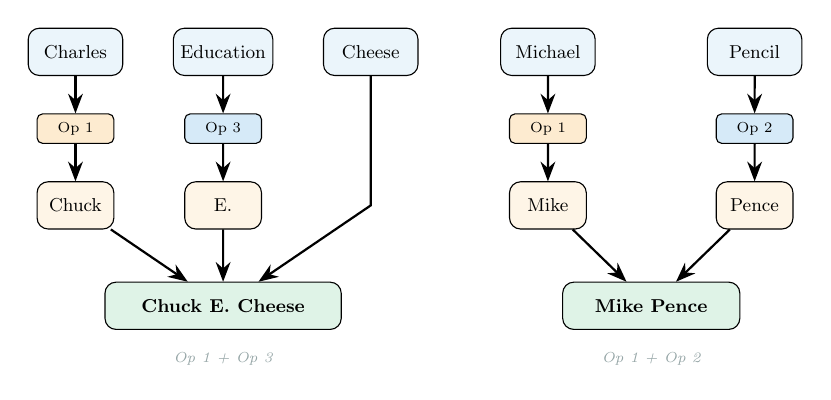
\begin{tikzpicture}[
  scale=0.75, transform shape,
  box/.style={draw, rounded corners=4pt, minimum height=0.8cm, font=\small,
              minimum width=1.6cm, align=center},
  opbox/.style={draw, rounded corners=2pt, minimum height=0.5cm, font=\scriptsize,
                fill=chill!15, minimum width=1.3cm},
  arr/.style={-{Stealth[length=2.5mm]}, thick}
]
  % Charles Education Cheese -> Chuck E. Cheese
  \node[box, fill=accent!10] (charles) at (0, 2.5) {Charles};
  \node[box, fill=accent!10] (education) at (2.5, 2.5) {Education};
  \node[box, fill=accent!10] (cheese) at (5, 2.5) {Cheese};

  \node[opbox, fill=backbone!20] (op1a) at (0, 1.2) {Op 1};
  \node[opbox, fill=accent!20] (op3a) at (2.5, 1.2) {Op 3};

  \node[box, fill=backbone!10, minimum width=1.3cm] (chuck) at (0, -0.1) {Chuck};
  \node[box, fill=backbone!10, minimum width=1.3cm] (ee) at (2.5, -0.1) {E.};

  \node[box, fill=circuit!15, minimum width=4cm] (cec) at (2.5, -1.8) {\textbf{Chuck E. Cheese}};

  \draw[arr] (charles) -- (op1a);
  \draw[arr] (op1a) -- (chuck);
  \draw[arr] (education) -- (op3a);
  \draw[arr] (op3a) -- (ee);
  \draw[arr] (chuck) -- (cec);
  \draw[arr] (ee) -- (cec);
  \draw[arr] (cheese) -- (5, -0.1) -- (cec);

  \node[font=\scriptsize\itshape, chill] at (2.5, -2.7) {Op 1 + Op 3};

  % Michael Pencil -> Mike Pence
  \node[box, fill=accent!10] (michael) at (8, 2.5) {Michael};
  \node[box, fill=accent!10] (pencil) at (11.5, 2.5) {Pencil};

  \node[opbox, fill=backbone!20] (op1b) at (8, 1.2) {Op 1};
  \node[opbox, fill=accent!20] (op2b) at (11.5, 1.2) {Op 2};

  \node[box, fill=backbone!10, minimum width=1.3cm] (mike) at (8, -0.1) {Mike};
  \node[box, fill=backbone!10, minimum width=1.3cm] (pence) at (11.5, -0.1) {Pence};

  \node[box, fill=circuit!15, minimum width=3cm] (mikepence) at (9.75, -1.8) {\textbf{Mike Pence}};

  \draw[arr] (michael) -- (op1b);
  \draw[arr] (op1b) -- (mike);
  \draw[arr] (pencil) -- (op2b);
  \draw[arr] (op2b) -- (pence);
  \draw[arr] (mike) -- (mikepence);
  \draw[arr] (pence) -- (mikepence);

  \node[font=\scriptsize\itshape, chill] at (9.75, -2.7) {Op 1 + Op 2};
\end{tikzpicture}
\end{center}

\vspace{0.3em}
Two independent shortenings in parallel --- the model must coordinate \textbf{two sub-circuits} that each transform a different input token.
\end{frame}

% =============================================
\begin{frame}{Chained operations: double shortening + fusion}

\begin{center}
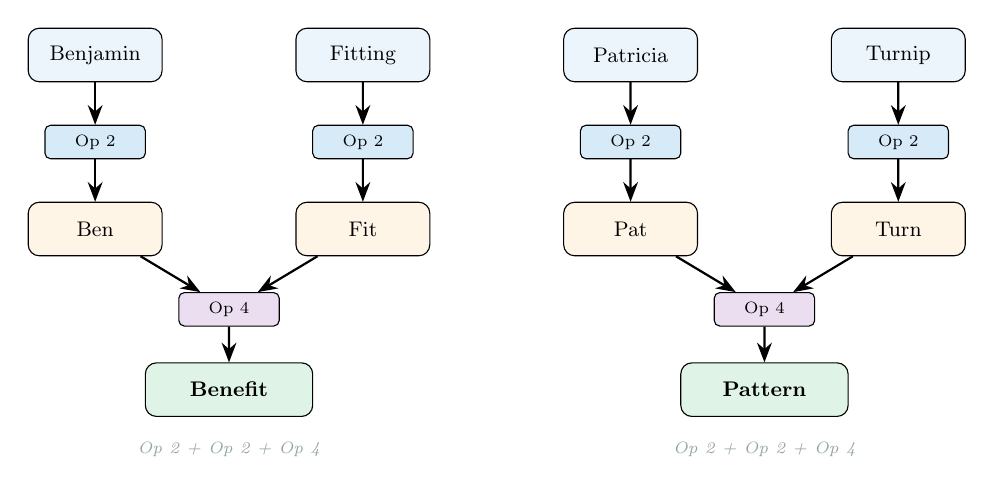
\begin{tikzpicture}[
  scale=0.85, transform shape,
  box/.style={draw, rounded corners=4pt, minimum height=0.8cm, font=\small,
              minimum width=2cm, align=center},
  opbox/.style={draw, rounded corners=2pt, minimum height=0.5cm, font=\scriptsize,
                fill=chill!15, minimum width=1.5cm},
  arr/.style={-{Stealth[length=2.5mm]}, thick}
]
  % Benjamin Fitting -> Benefit
  \node[box, fill=accent!10] (benjamin) at (0, 2.5) {Benjamin};
  \node[box, fill=accent!10] (fitting) at (4, 2.5) {Fitting};

  \node[opbox, fill=accent!20] (op2a) at (0, 1.2) {Op 2};
  \node[opbox, fill=accent!20] (op2b) at (4, 1.2) {Op 2};

  \node[box, fill=backbone!10] (ben) at (0, -0.1) {Ben};
  \node[box, fill=backbone!10] (fit) at (4, -0.1) {Fit};

  \node[opbox, fill=fusion!20] (op4a) at (2, -1.3) {Op 4};
  \node[box, fill=circuit!15, minimum width=2.5cm] (benefit) at (2, -2.5) {\textbf{Benefit}};

  \draw[arr] (benjamin) -- (op2a);
  \draw[arr] (op2a) -- (ben);
  \draw[arr] (fitting) -- (op2b);
  \draw[arr] (op2b) -- (fit);
  \draw[arr] (ben) -- (op4a);
  \draw[arr] (fit) -- (op4a);
  \draw[arr] (op4a) -- (benefit);

  \node[font=\scriptsize\itshape, chill] at (2, -3.4) {Op 2 + Op 2 + Op 4};

  % Patricia Turnip -> Pattern
  \node[box, fill=accent!10] (patricia) at (8, 2.5) {Patricia};
  \node[box, fill=accent!10] (turnip) at (12, 2.5) {Turnip};

  \node[opbox, fill=accent!20] (op2c) at (8, 1.2) {Op 2};
  \node[opbox, fill=accent!20] (op2d) at (12, 1.2) {Op 2};

  \node[box, fill=backbone!10] (pat) at (8, -0.1) {Pat};
  \node[box, fill=backbone!10] (turn) at (12, -0.1) {Turn};

  \node[opbox, fill=fusion!20] (op4b) at (10, -1.3) {Op 4};
  \node[box, fill=circuit!15, minimum width=2.5cm] (pattern) at (10, -2.5) {\textbf{Pattern}};

  \draw[arr] (patricia) -- (op2c);
  \draw[arr] (op2c) -- (pat);
  \draw[arr] (turnip) -- (op2d);
  \draw[arr] (op2d) -- (turn);
  \draw[arr] (pat) -- (op4b);
  \draw[arr] (turn) -- (op4b);
  \draw[arr] (op4b) -- (pattern);

  \node[font=\scriptsize\itshape, chill] at (10, -3.4) {Op 2 + Op 2 + Op 4};
\end{tikzpicture}
\end{center}

\vspace{0.3em}
Three operations composed: two parallel shortenings feed into a fusion step. The model must coordinate \textbf{three independent sub-circuits} in a single forward pass.
\end{frame}

% =============================================
% PART 2 DIVIDER
% =============================================
\begin{frame}[plain,noframenumbering]
\begin{center}
\vfill
  {\setlength{\fboxrule}{2.5pt}\fcolorbox{black}{white}{\parbox{0.7\textwidth}{\centering\vspace{0.8em}
    {\Large\bfseries Part 2: Methods}
  \vspace{0.8em}}}}
\vfill
\end{center}
\end{frame}

% =============================================
% DATASETS
% =============================================
\begin{frame}{Minimal-pair datasets}
\hypertarget{sl:datasets}{}

Each pair follows \href{https://arxiv.org/abs/1912.00582}{BLiMP} format {\scriptsize(Warstadt et al., 2020)}: \texttt{\{good, bad, target\_token, foil\_token\}}

\vspace{0.5em}
\begin{center}
\footnotesize
\begin{tabular}{lll}
\toprule
\textbf{Operation} & \textbf{Good prompt} & \textbf{Target / Foil} \\
\midrule
Op 1 & ``People call Robert by the name'' & Bob / Mark \\
Op 2 & ``Timothy goes by'' & Tim / Tom \\
Op 3 & ``The letter J is pronounced'' & Jay / Gee \\
Op 4 & ``Bill Ding sounds like'' & building / nothing \\
Op 5 & ``Neil sounds like'' & kneel / wheel \\
Op 6 & ``The word curtain contains the name'' & Curt / nothing \\
\bottomrule
\end{tabular}
\end{center}

\vspace{0.5em}
\textbf{Evaluation:} logit difference at final position.

\textbf{Gate:} $>$70\% accuracy before circuit discovery.

\vspace{0.5em}
Ops 2, 3, 5 are procedurally expandable (\href{http://www.speech.cs.cmu.edu/cgi-bin/cmudict}{CMU Pronouncing Dictionary}).\\
Ops 1, 4, 6 are controlled vocabularies.
\end{frame}

% =============================================
% EXAMPLES
% =============================================
\begin{frame}{The dataset: selected examples}

\begin{center}
\renewcommand{\arraystretch}{1.3}
\begin{tabular}{lll}
\toprule
\textbf{Input} & \textbf{Target} & \textbf{Operation} \\
\midrule
William Ding & Building & Op 1 + Op 4 \\
William Ding & Building & Op 1 + Op 4 \\
Richard Tater & Dictator & Op 1 + Op 4 \\
Charles Education Cheese & Chuck E. Cheese & Op 1 + Op 3 \\
Timothy Bermuda & Timber & Op 2 + Op 2 + Op 4 \\
\midrule
Bill Ding & Building & Op 4 only \\
Justin Time & Just in time & Op 4 only \\
Brock Lee & Broccoli & Op 4 only \\
Barb Dwyer & Barbed wire & Op 4 only \\
\midrule
Sue Permarket & Supermarket & Op 4 only \\
Al Gorithm & Algorithm & Op 4 only \\
\bottomrule
\end{tabular}
\end{center}

\vspace{0.3em}
{\small 99 oronym pairs, 32 hypocorism pairs, 120 homophone pairs --- 446 total minimal pairs across 6 operations.}
\end{frame}

% =============================================
% TOKENIZATION AUDIT
% =============================================
\begin{frame}{Tokenization audit}

BPE tokenization can break phonological tasks:

\vspace{0.5em}
\begin{center}
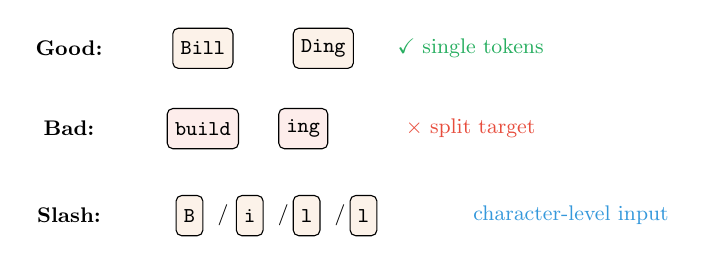
\begin{tikzpicture}[
  scale=0.85, transform shape,
  tok/.style={draw, rounded corners=2pt, minimum height=0.6cm, font=\ttfamily\small,
              fill=tok!10},
  bad/.style={draw, rounded corners=2pt, minimum height=0.6cm, font=\ttfamily\small,
              fill=phoneme!10}
]
  % Good tokenization
  \node[font=\small\bfseries] at (-2, 1) {Good:};
  \node[tok] (g1) at (0, 1) {Bill};
  \node[tok] (g2) at (1.8, 1) {Ding};
  \node[font=\small, circuit] at (4, 1) {$\checkmark$ single tokens};

  % Bad tokenization
  \node[font=\small\bfseries] at (-2, -0.2) {Bad:};
  \node[bad] (b1) at (0, -0.2) {build};
  \node[bad] (b2) at (1.5, -0.2) {ing};
  \node[font=\small, phoneme] at (4, -0.2) {$\times$ split target};

  % Slash condition
  \node[font=\small\bfseries] at (-2, -1.5) {Slash:};
  \node[tok] (s1) at (-0.2, -1.5) {B};
  \node[font=\small] at (0.3, -1.5) {/};
  \node[tok] (s2) at (0.7, -1.5) {i};
  \node[font=\small] at (1.2, -1.5) {/};
  \node[tok] (s3) at (1.55, -1.5) {l};
  \node[font=\small] at (2.05, -1.5) {/};
  \node[tok] (s4) at (2.4, -1.5) {l};
  \node[font=\small, accent] at (5.5, -1.5) {character-level input};
\end{tikzpicture}
\end{center}

\vspace{0.5em}
Following \href{https://aclanthology.org/2026.latechclfl-1.9}{Liao \& Shi (2026)}: if slash-delimited input improves Op 4 accuracy, the circuit \emph{exists} but is bottlenecked by tokenization.

\vspace{0.5em}
$\Rightarrow$ Distinguishes tokenization bottleneck from missing circuit.
\end{frame}

% =============================================
% CIRCUIT DISCOVERY
% =============================================
\begin{frame}{Standard Mechanistic Interpretability Pipeline}
\hypertarget{sl:discovery}{}

\begin{center}
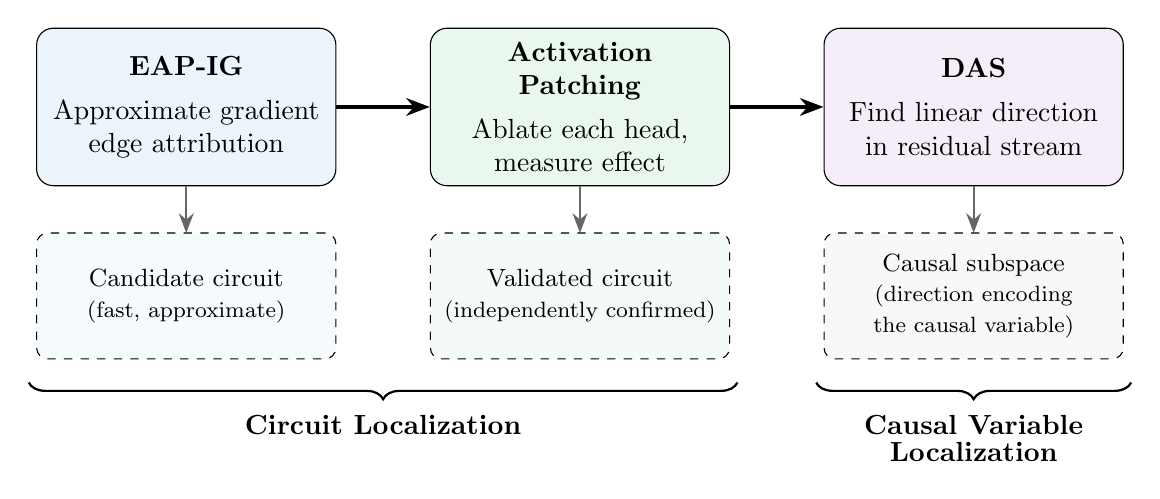
\begin{tikzpicture}[
  method/.style={draw, rounded corners=6pt, minimum height=2cm, minimum width=3.8cm,
               align=center, font=\normalsize},
  output/.style={draw, dashed, rounded corners=4pt, minimum height=1.6cm, minimum width=3.8cm,
               align=center, font=\small},
  arr/.style={-{Stealth[length=3mm]}, very thick, black},
  downarr/.style={-{Stealth[length=2.5mm]}, thick, black!60}
]
  % Top row: methods
  \node[method, fill=accent!10] (eap) at (0, 2) {
    \textbf{EAP-IG}\\[4pt]
    Approximate gradient\\
    edge attribution
  };

  \node[method, fill=circuit!10] (ap) at (5, 2) {
    \textbf{Activation}\\
    \textbf{Patching}\\[4pt]
    Ablate each head,\\
    measure effect
  };

  \node[method, fill=fusion!10] (das) at (10, 2) {
    \textbf{DAS}\\[4pt]
    Find linear direction\\
    in residual stream
  };

  % Arrows between methods
  \draw[arr] (eap) -- (ap);
  \draw[arr] (ap) -- (das);

  % Down arrows
  \draw[downarr] (eap) -- (0, 0.4);
  \draw[downarr] (ap) -- (5, 0.4);
  \draw[downarr] (das) -- (10, 0.4);

  % Bottom row: outputs
  \node[output, fill=accent!5] at (0, -0.4) {
    Candidate circuit\\
    {\footnotesize (fast, approximate)}
  };

  \node[output, fill=circuit!5] at (5, -0.4) {
    Validated circuit\\
    {\footnotesize (independently confirmed)}
  };

  \node[output, fill=fusion!5] at (10, -0.4) {
    Causal subspace\\
    {\footnotesize (direction encoding}\\
    {\footnotesize the causal variable)}
  };

  % Braces
  \draw[decorate, decoration={brace, amplitude=6pt, mirror}, thick]
    (-2, -1.5) -- (7, -1.5) node[midway, below=8pt, font=\normalsize\bfseries] {Circuit Localization};
  \draw[decorate, decoration={brace, amplitude=6pt, mirror}, thick]
    (8, -1.5) -- (12, -1.5) node[midway, below=8pt, font=\normalsize\bfseries, align=center] {Causal Variable\\[-2pt]Localization};

\end{tikzpicture}
\end{center}

\vspace{0.3em}
{\scriptsize Following the MIB framework (\href{https://arxiv.org/abs/2504.13151}{Mueller et al., 2025}): discover circuits via attribution, validate with interventions, localize causal variables.}
\end{frame}

% =============================================
% PART 3 DIVIDER
% =============================================
\begin{frame}[plain,noframenumbering]
\begin{center}
\vfill
  {\setlength{\fboxrule}{2.5pt}\fcolorbox{black}{white}{\parbox{0.7\textwidth}{\centering\vspace{0.8em}
    {\Large\bfseries Part 3: Hypotheses}
  \vspace{0.8em}}}}
\vfill
\end{center}
\end{frame}

% =============================================
% BACKBONE HYPOTHESIS
% =============================================
\begin{frame}{Prior circuits converge on the same layers}
\hypertarget{sl:backbone}{}

Known GPT-2 circuits reuse the \textbf{same layers} across unrelated tasks:

\vspace{0.2em}
\begin{center}
\scriptsize
\renewcommand{\arraystretch}{1.1}
\begin{tabular}{lll}
\toprule
\textbf{Task} & \textbf{Key heads (layers)} & \textbf{Source} \\
\midrule
IOI & S-inhibition (L7--8), name movers (L9--10) & \href{https://arxiv.org/abs/2211.00593}{Wang et al.\ 2023} \\
Greater-than & Attn (L5--9), MLPs (L8--11) & \href{https://arxiv.org/abs/2305.00586}{Hanna et al.\ 2023} \\
Induction & Prev-token (L2, L4), induction (L5--7) & \href{https://arxiv.org/abs/2209.11895}{Olsson et al.\ 2022} \\
SVA & Top heads span L0, L6, L9--11 & \href{https://arxiv.org/abs/2506.22105}{Africa, 2025} \\
\bottomrule
\end{tabular}
\end{center}

\vspace{0.3em}
\begin{center}
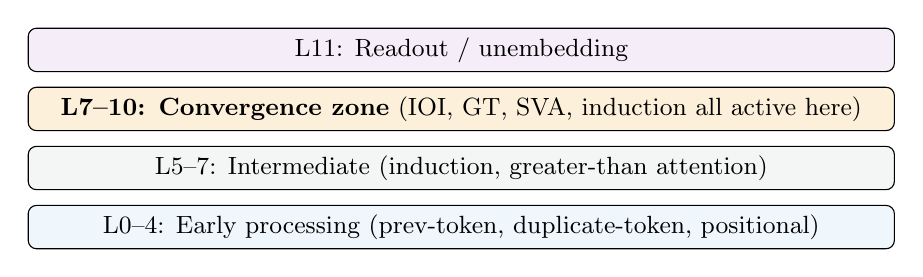
\begin{tikzpicture}[
  layer/.style={draw, rounded corners=3pt, minimum height=0.55cm, font=\small,
                minimum width=11cm},
]
  \node[layer, fill=accent!8] at (0, 0) {L0--4: Early processing (prev-token, duplicate-token, positional)};
  \node[layer, fill=chill!10] at (0, 0.75) {L5--7: Intermediate (induction, greater-than attention)};
  \node[layer, fill=backbone!15] at (0, 1.5) {\textbf{L7--10: Convergence zone} (IOI, GT, SVA, induction all active here)};
  \node[layer, fill=fusion!10] at (0, 2.25) {L11: Readout / unembedding};
\end{tikzpicture}
\end{center}

\vspace{0.4em}
Layers 7--10 are GPT-2's general-purpose computation engine. Does this extend to phonology?
\end{frame}

% =============================================
% FUSION HEADS
% =============================================
\begin{frame}{Three hypotheses}
\hypertarget{sl:fusionheads}{}

\begin{center}
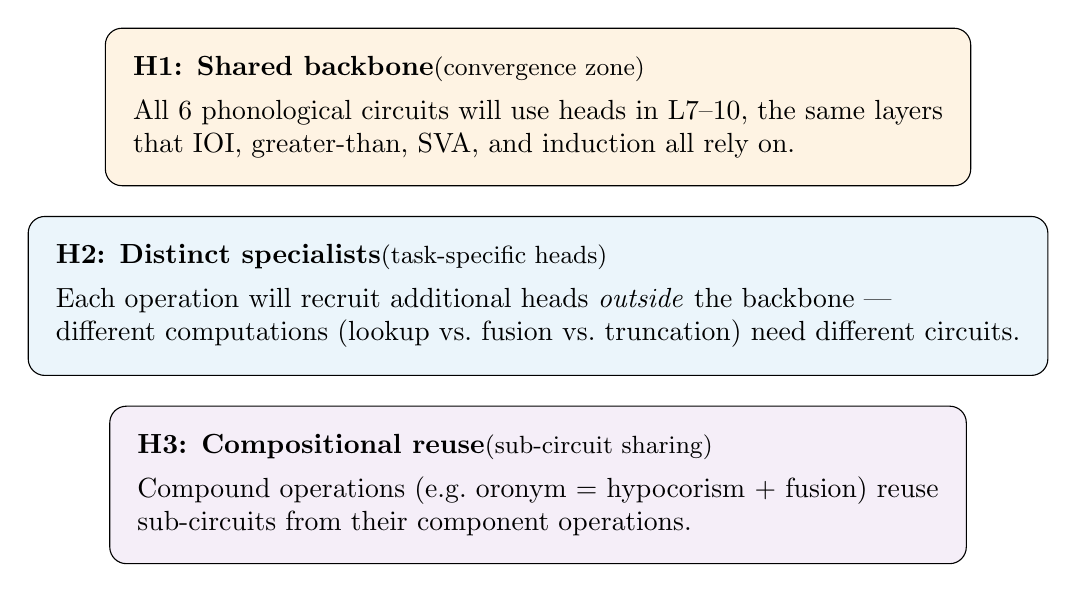
\begin{tikzpicture}[
  hyp/.style={draw, rounded corners=6pt, minimum height=2cm, minimum width=10.5cm,
              align=left, font=\normalsize, inner sep=10pt},
]
  \node[hyp, fill=backbone!12] at (0, 4.2) {
    \textbf{H1: Shared backbone}\hfill{\small (convergence zone)}\\[4pt]
    All 6 phonological circuits will use heads in L7--10, the same layers\\
    that IOI, greater-than, SVA, and induction all rely on.
  };

  \node[hyp, fill=accent!10] at (0, 1.8) {
    \textbf{H2: Distinct specialists}\hfill{\small (task-specific heads)}\\[4pt]
    Each operation will recruit additional heads \emph{outside} the backbone ---\\
    different computations (lookup vs.\ fusion vs.\ truncation) need different circuits.
  };

  \node[hyp, fill=fusion!10] at (0, -0.6) {
    \textbf{H3: Compositional reuse}\hfill{\small (sub-circuit sharing)}\\[4pt]
    Compound operations (e.g.\ oronym = hypocorism + fusion) reuse\\
    sub-circuits from their component operations.
  };
\end{tikzpicture}
\end{center}
\end{frame}

% =============================================
% COMPOSITION
% =============================================
\begin{frame}{Compositional validation protocol}
\hypertarget{sl:composition}{}

\begin{center}
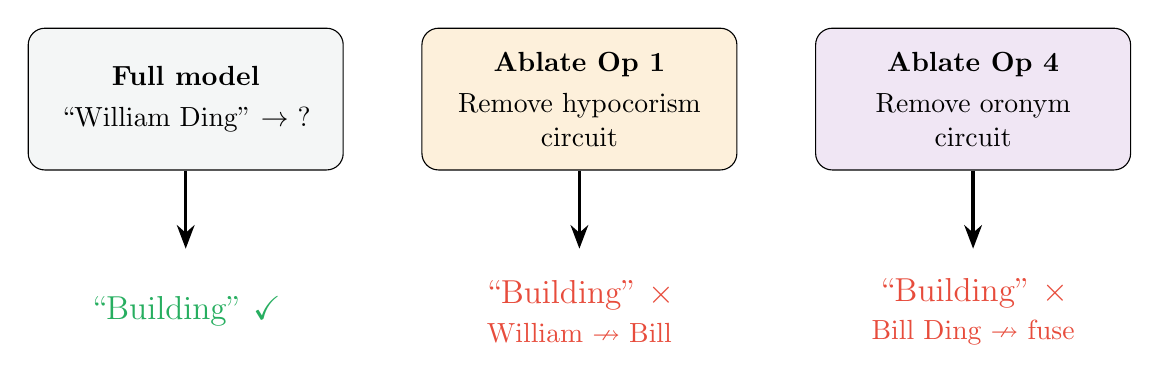
\begin{tikzpicture}[
  test/.style={draw, rounded corners=6pt, minimum height=1.8cm, minimum width=4cm,
               align=center, font=\normalsize},
  result/.style={font=\normalsize, align=center},
  arr/.style={-{Stealth[length=3mm]}, very thick, black}
]
  % Tests
  \node[test, fill=chill!10] (full) at (0, 2.5) {
    \textbf{Full model}\\[3pt]
    ``William Ding'' $\to$ ?
  };

  \node[test, fill=backbone!15] (abl1) at (5, 2.5) {
    \textbf{Ablate Op 1}\\[3pt]
    Remove hypocorism\\
    circuit
  };

  \node[test, fill=fusion!15] (abl4) at (10, 2.5) {
    \textbf{Ablate Op 4}\\[3pt]
    Remove oronym\\
    circuit
  };

  % Expected results
  \node[result, circuit] at (0, -0.2) {\large ``Building'' $\checkmark$};
  \node[result, phoneme] at (5, -0.2) {\large ``Building'' $\times$\\[2pt] William $\nrightarrow$ Bill};
  \node[result, phoneme] at (10, -0.2) {\large ``Building'' $\times$\\[2pt] Bill Ding $\nrightarrow$ fuse};

  \draw[arr] (full) -- (0, 0.6);
  \draw[arr] (abl1) -- (5, 0.6);
  \draw[arr] (abl4) -- (10, 0.6);
\end{tikzpicture}
\end{center}

\vspace{0.3em}
{\large Each component circuit is \textbf{independently necessary}.}

{\large $\to$ True compositional structure, not a single monolithic circuit.}
\end{frame}

% =============================================
% RESULTS — CIRCUIT LOCALIZATION DIVIDER
% =============================================
\begin{frame}[plain,noframenumbering]
\hypertarget{sl:results}{}
\begin{center}
\vfill
  {\setlength{\fboxrule}{2.5pt}\fcolorbox{black}{white}{\parbox{0.7\textwidth}{\centering\vspace{0.8em}
    {\Large\bfseries Part 4: Circuit Localization}\\[4pt]
    {\normalsize Which components matter?}
  \vspace{0.8em}}}}
\vfill
\end{center}
\end{frame}

% =============================================
% BEHAVIORAL VALIDATION
% =============================================
\begin{frame}{Behavioral validation: GPT-2 can do phonology}
\hypertarget{sl:behavioral}{}

All six operations pass the 70\% accuracy gate on \href{https://cdn.openai.com/better-language-models/language_models_are_unsupervised_multitask_learners.pdf}{GPT-2} (Radford et al., 2019; 117M):

\vspace{0.5em}
\begin{center}
\small
\renewcommand{\arraystretch}{1.2}
\begin{tabular}{llccc}
\toprule
\textbf{Op} & \textbf{Task} & \textbf{N} & \textbf{Accuracy} & \textbf{Mean logit diff} \\
\midrule
1 & Hypocorism & 132 & 90.9\% & 1.67 \\
2 & Clipping & 62 & 93.5\% & 1.80 \\
3 & Initialism & 68 & 70.6\% & 0.58 \\
\rowcolor{fusion!8}
4 & \textbf{Oronym} & \textbf{104} & \textbf{73.1\%} & \textbf{1.26} \\
5 & Homophone & 52 & 92.3\% & 2.78 \\
6 & Folk etymology & 64 & 100.0\% & 3.21 \\
\bottomrule
\end{tabular}
\end{center}

\vspace{0.5em}
Op 3 (initialism) is weakest --- letter-to-phoneme-name is the hardest regular rule.

Op 6 (folk etymology) is perfect --- ``curtain $\to$ Curt'' is trivially compositional.

\textbf{Conclusion:} GPT-2 has phonological knowledge we can circuit-hunt for.
\end{frame}

% =============================================
% EAP-IG RESULTS
% =============================================
\begin{frame}{EAP-IG circuit discovery}
\hypertarget{sl:eapresults}{}

\small
Ran \href{https://arxiv.org/abs/2310.10348}{edge attribution patching with integrated gradients} (EAP-IG; Syed et al., 2023) per task.

\vspace{0.3em}
\textbf{Quality:} all circuits are faithful (CMD $<$ 0.08, CPR $\approx$ 1.0).

\vspace{0.5em}
\begin{center}
\renewcommand{\arraystretch}{1.15}
\begin{tabular}{llcc}
\toprule
\textbf{Op} & \textbf{Task} & \textbf{CMD $\downarrow$} & \textbf{CPR $\uparrow$} \\
\midrule
1 & Hypocorism & 0.018 & 1.006 \\
2 & Clipping & 0.019 & 1.007 \\
3 & Initialism & 0.060 & 1.043 \\
\rowcolor{fusion!8}
4 & \textbf{Oronym} & \textbf{0.047} & \textbf{1.006} \\
5 & Homophone & 0.025 & 0.999 \\
6 & Folk etymology & 0.072 & 1.063 \\
\bottomrule
\end{tabular}
\end{center}

\vspace{0.5em}
{\footnotesize CMD = circuit minimality distance (lower = sparser, better).\\
CPR = circuit precision-recall (1.0 = perfect; $>$1.0 = slight over-recovery is OK).}
\end{frame}

% =============================================
% TOP EDGES
% =============================================
\begin{frame}{What the circuits look like}

\small
Top attribution edges reveal shared structure across tasks:

\vspace{0.5em}
\begin{columns}[T]
\begin{column}{0.47\textwidth}
\textbf{Shared across all tasks:}
\begin{itemize}
  \item \texttt{input $\to$ m0}: token embeddings feed MLP-0 (highest score in 5/6 tasks)
  \item \texttt{m0 $\to$ m1}: MLP-0 $\to$ MLP-1 chain
  \item \texttt{a10.h10 $\to$ logits}: late readout
\end{itemize}

\vspace{0.5em}
\textbf{This is the backbone:} early MLPs and late attention heads appear in every phonological circuit.
\end{column}

\begin{column}{0.47\textwidth}
\textbf{Task-specific differences:}
\begin{itemize}
  \item Op 1: \texttt{a10.h0}, \texttt{a10.h6} dominate (name movers?)
  \item Op 4: \texttt{a9.h9} ranks high (cross-boundary fusion?)
  \item Op 5: \texttt{a8.h11} is strongest non-MLP edge (phoneme identity?)
  \item Op 6: \texttt{a10.h1} appears (creative composition?)
\end{itemize}

\vspace{0.5em}
\textbf{Distinct mid-layer heads} per operation $\Rightarrow$ distinct circuits.
\end{column}
\end{columns}
\end{frame}

% =============================================
% PART 5 DIVIDER — CIRCUIT VALIDATION
% =============================================
\begin{frame}[plain,noframenumbering]
\hypertarget{sl:validation}{}
\begin{center}
\vfill
  {\setlength{\fboxrule}{2.5pt}\fcolorbox{black}{white}{\parbox{0.7\textwidth}{\centering\vspace{0.8em}
    {\Large\bfseries Part 5: Circuit Validation}\\[4pt]
    {\normalsize Does the evidence hold up independently?}
  \vspace{0.8em}}}}
\vfill
\end{center}
\end{frame}

% =============================================
% CIRCUIT OVERLAP MATRIX — PREDICTION vs RESULTS
% =============================================
\begin{frame}{Circuit overlap matrix --- prediction vs.\ results}

\begin{columns}[T]
\begin{column}{0.47\textwidth}
\begin{center}
\textbf{Predicted}\\[4pt]
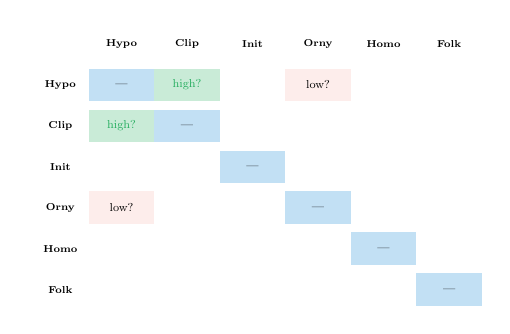
\begin{tikzpicture}[scale=0.52, transform shape,
  cell/.style={minimum width=1.6cm, minimum height=0.8cm, font=\footnotesize, align=center},
  hdr/.style={font=\bfseries\scriptsize, minimum width=1.6cm, minimum height=0.8cm}
]
  \node[hdr] at (1.8, 0) {Hypo};
  \node[hdr] at (3.4, 0) {Clip};
  \node[hdr] at (5.0, 0) {Init};
  \node[hdr] at (6.6, 0) {Orny};
  \node[hdr] at (8.2, 0) {Homo};
  \node[hdr] at (9.8, 0) {Folk};

  \node[hdr, right] at (-0.5, -1) {Hypo};
  \node[hdr, right] at (-0.5, -2) {Clip};
  \node[hdr, right] at (-0.5, -3) {Init};
  \node[hdr, right] at (-0.5, -4) {Orny};
  \node[hdr, right] at (-0.5, -5) {Homo};
  \node[hdr, right] at (-0.5, -6) {Folk};

  \fill[accent!30] (1.0,-0.6) rectangle (2.6,-1.4); \node[cell] at (1.8,-1) {---};
  \fill[accent!30] (2.6,-1.6) rectangle (4.2,-2.4); \node[cell] at (3.4,-2) {---};
  \fill[accent!30] (4.2,-2.6) rectangle (5.8,-3.4); \node[cell] at (5.0,-3) {---};
  \fill[accent!30] (5.8,-3.6) rectangle (7.4,-4.4); \node[cell] at (6.6,-4) {---};
  \fill[accent!30] (7.4,-4.6) rectangle (9.0,-5.4); \node[cell] at (8.2,-5) {---};
  \fill[accent!30] (9.0,-5.6) rectangle (10.6,-6.4); \node[cell] at (9.8,-6) {---};

  \fill[circuit!25] (2.6,-0.6) rectangle (4.2,-1.4); \node[cell, circuit] at (3.4,-1) {high?};
  \fill[circuit!25] (1.0,-1.6) rectangle (2.6,-2.4); \node[cell, circuit] at (1.8,-2) {high?};

  \fill[phoneme!10] (5.8,-0.6) rectangle (7.4,-1.4); \node[cell, black] at (6.6,-1) {low?};
  \fill[phoneme!10] (1.0,-3.6) rectangle (2.6,-4.4); \node[cell, black] at (1.8,-4) {low?};
\end{tikzpicture}
\end{center}
\end{column}

\begin{column}{0.53\textwidth}
\begin{center}
\textbf{Observed (EAP-IG, top 30 heads)}\\[4pt]
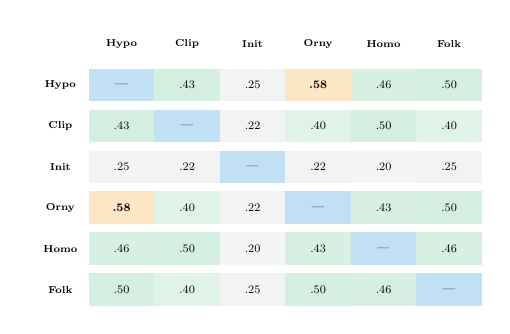
\begin{tikzpicture}[scale=0.52, transform shape,
  cell/.style={minimum width=1.6cm, minimum height=0.8cm, font=\footnotesize, align=center},
  hdr/.style={font=\bfseries\scriptsize, minimum width=1.6cm, minimum height=0.8cm}
]
  \node[hdr] at (1.8, 0) {Hypo};
  \node[hdr] at (3.4, 0) {Clip};
  \node[hdr] at (5.0, 0) {Init};
  \node[hdr] at (6.6, 0) {Orny};
  \node[hdr] at (8.2, 0) {Homo};
  \node[hdr] at (9.8, 0) {Folk};

  \node[hdr, right] at (-0.5, -1) {Hypo};
  \node[hdr, right] at (-0.5, -2) {Clip};
  \node[hdr, right] at (-0.5, -3) {Init};
  \node[hdr, right] at (-0.5, -4) {Orny};
  \node[hdr, right] at (-0.5, -5) {Homo};
  \node[hdr, right] at (-0.5, -6) {Folk};

  % Diagonal
  \fill[accent!30] (1.0,-0.6) rectangle (2.6,-1.4); \node[cell] at (1.8,-1) {---};
  \fill[accent!30] (2.6,-1.6) rectangle (4.2,-2.4); \node[cell] at (3.4,-2) {---};
  \fill[accent!30] (4.2,-2.6) rectangle (5.8,-3.4); \node[cell] at (5.0,-3) {---};
  \fill[accent!30] (5.8,-3.6) rectangle (7.4,-4.4); \node[cell] at (6.6,-4) {---};
  \fill[accent!30] (7.4,-4.6) rectangle (9.0,-5.4); \node[cell] at (8.2,-5) {---};
  \fill[accent!30] (9.0,-5.6) rectangle (10.6,-6.4); \node[cell] at (9.8,-6) {---};

  % Row 1 (Hypo)
  \fill[circuit!20] (2.6,-0.6) rectangle (4.2,-1.4); \node[cell] at (3.4,-1) {.43};
  \fill[chill!12] (4.2,-0.6) rectangle (5.8,-1.4); \node[cell] at (5.0,-1) {.25};
  \fill[backbone!25] (5.8,-0.6) rectangle (7.4,-1.4); \node[cell, font=\footnotesize\bfseries] at (6.6,-1) {.58};
  \fill[circuit!18] (7.4,-0.6) rectangle (9.0,-1.4); \node[cell] at (8.2,-1) {.46};
  \fill[circuit!20] (9.0,-0.6) rectangle (10.6,-1.4); \node[cell] at (9.8,-1) {.50};
  % Row 2 (Clip)
  \fill[circuit!20] (1.0,-1.6) rectangle (2.6,-2.4); \node[cell] at (1.8,-2) {.43};
  \fill[chill!12] (4.2,-1.6) rectangle (5.8,-2.4); \node[cell] at (5.0,-2) {.22};
  \fill[circuit!15] (5.8,-1.6) rectangle (7.4,-2.4); \node[cell] at (6.6,-2) {.40};
  \fill[circuit!20] (7.4,-1.6) rectangle (9.0,-2.4); \node[cell] at (8.2,-2) {.50};
  \fill[circuit!15] (9.0,-1.6) rectangle (10.6,-2.4); \node[cell] at (9.8,-2) {.40};
  % Row 3 (Init)
  \fill[chill!12] (1.0,-2.6) rectangle (2.6,-3.4); \node[cell] at (1.8,-3) {.25};
  \fill[chill!12] (2.6,-2.6) rectangle (4.2,-3.4); \node[cell] at (3.4,-3) {.22};
  \fill[chill!12] (5.8,-2.6) rectangle (7.4,-3.4); \node[cell] at (6.6,-3) {.22};
  \fill[chill!10] (7.4,-2.6) rectangle (9.0,-3.4); \node[cell] at (8.2,-3) {.20};
  \fill[chill!12] (9.0,-2.6) rectangle (10.6,-3.4); \node[cell] at (9.8,-3) {.25};
  % Row 4 (Orny)
  \fill[backbone!25] (1.0,-3.6) rectangle (2.6,-4.4); \node[cell, font=\footnotesize\bfseries] at (1.8,-4) {.58};
  \fill[circuit!15] (2.6,-3.6) rectangle (4.2,-4.4); \node[cell] at (3.4,-4) {.40};
  \fill[chill!12] (4.2,-3.6) rectangle (5.8,-4.4); \node[cell] at (5.0,-4) {.22};
  \fill[circuit!18] (7.4,-3.6) rectangle (9.0,-4.4); \node[cell] at (8.2,-4) {.43};
  \fill[circuit!20] (9.0,-3.6) rectangle (10.6,-4.4); \node[cell] at (9.8,-4) {.50};
  % Row 5 (Homo)
  \fill[circuit!18] (1.0,-4.6) rectangle (2.6,-5.4); \node[cell] at (1.8,-5) {.46};
  \fill[circuit!20] (2.6,-4.6) rectangle (4.2,-5.4); \node[cell] at (3.4,-5) {.50};
  \fill[chill!10] (4.2,-4.6) rectangle (5.8,-5.4); \node[cell] at (5.0,-5) {.20};
  \fill[circuit!18] (5.8,-4.6) rectangle (7.4,-5.4); \node[cell] at (6.6,-5) {.43};
  \fill[circuit!18] (9.0,-4.6) rectangle (10.6,-5.4); \node[cell] at (9.8,-5) {.46};
  % Row 6 (Folk)
  \fill[circuit!20] (1.0,-5.6) rectangle (2.6,-6.4); \node[cell] at (1.8,-6) {.50};
  \fill[circuit!15] (2.6,-5.6) rectangle (4.2,-6.4); \node[cell] at (3.4,-6) {.40};
  \fill[chill!12] (4.2,-5.6) rectangle (5.8,-6.4); \node[cell] at (5.0,-6) {.25};
  \fill[circuit!20] (5.8,-5.6) rectangle (7.4,-6.4); \node[cell] at (6.6,-6) {.50};
  \fill[circuit!18] (7.4,-5.6) rectangle (9.0,-6.4); \node[cell] at (8.2,-6) {.46};
\end{tikzpicture}
\end{center}
\end{column}
\end{columns}

\vspace{0.3em}
\small
\textbf{H1} \checkmark{} 6 universal heads in all 6 circuits --- all in L8--11.\\
\textbf{H2} \checkmark{} Initialism most distinct ($J \leq 0.25$ with every other task).\\
\textbf{H3} ? \textbf{Surprise:} Oronym--Hypocorism is the \emph{highest} pair (0.58) --- we predicted low (different computations: fusion vs.\ lookup). High overlap is \emph{consistent with} compositional reuse, but needs mechanistic confirmation: do the shared heads perform the shortening step?
\end{frame}

% =============================================
% ZOOMING IN: HYPOCORISM–ORONYM OVERLAP
% =============================================
\begin{frame}{Zooming in: why is oronym--hypocorism overlap so high?}

\begin{center}
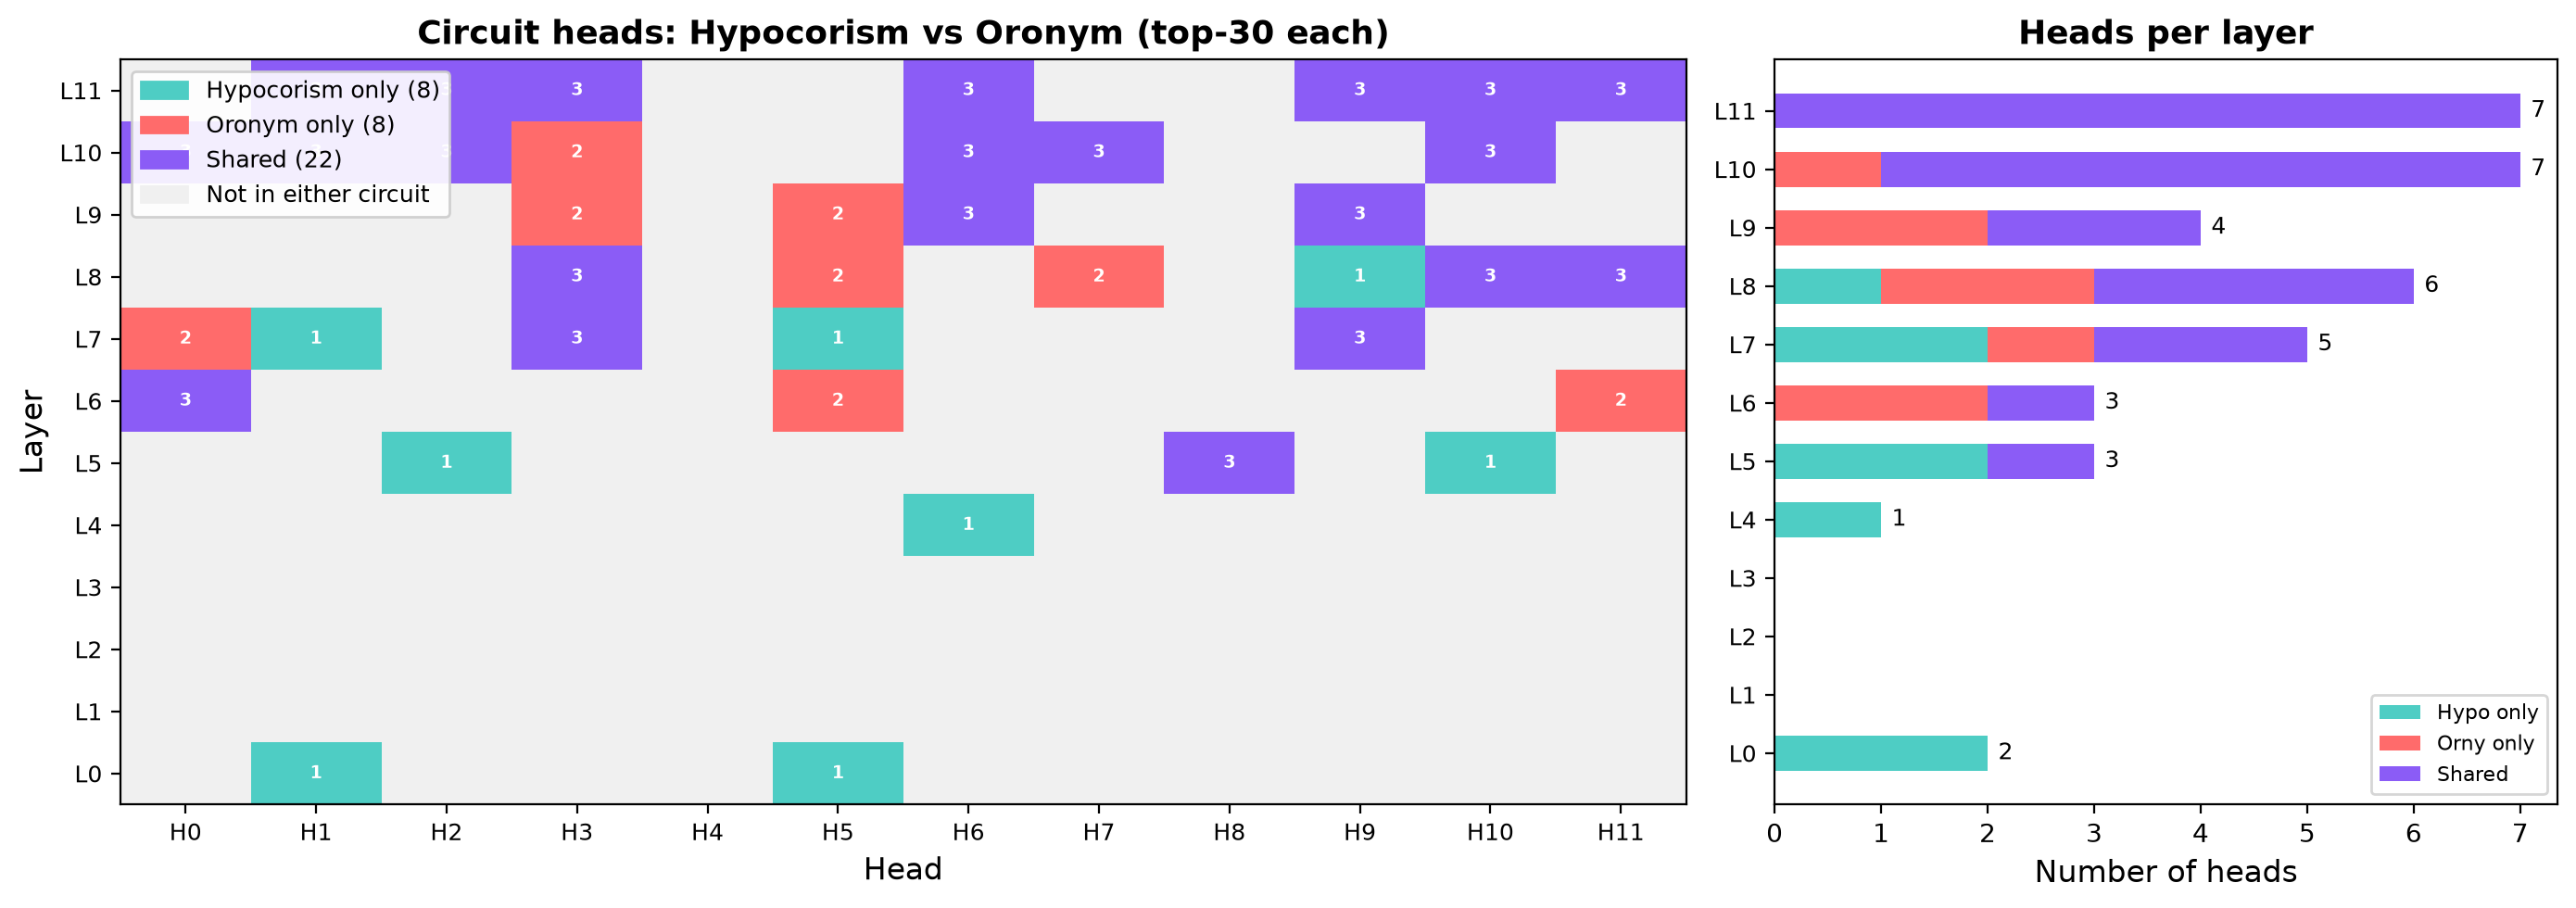
\includegraphics[width=0.95\textwidth]{figures/circuit_overlap_hypo_orny.png}
\end{center}

\vspace{0.3em}
{\small The oronym circuit contains \textbf{22 of 30} hypocorism heads. Shared heads concentrate in L10--11 (13/22). Oronym-only heads are in L6--10 --- plausibly the cross-boundary fusion step that oronyms require beyond shortening.}
\end{frame}

% =============================================
% WHAT WOULD CONFIRM COMPOSITIONAL REUSE?
% =============================================
\begin{frame}{Testing compositional reuse (H3)}

The overlap is \emph{consistent with} H3, but doesn't prove sequential computation. Three experiments that would:

\vspace{0.5em}
\begin{enumerate}
  \item \textbf{DAS probing at intermediate layers:} Train rank-1 DAS probes for ``shortening'' (Robert $\to$ Bob) at L8--9. If the oronym circuit activates these same directions before the fusion heads fire (L10--11), the chain is real.

  \item \textbf{Ablate the shared sub-circuit:} Knock out the 22 shared heads in the oronym circuit. If oronym accuracy drops to chance \emph{and} the failure mode looks like ``couldn't shorten the name'' (not ``couldn't fuse''), the oronym depends on the hypocorism sub-circuit specifically.

  \item \textbf{Cross-task activation patching:} Patch oronym activations at the 22 shared heads with hypocorism activations from a matched input. If oronym accuracy is preserved, the shared heads are functionally interchangeable.
\end{enumerate}

\vspace{0.3em}
{\small Status: planned. These require targeted DAS training and ablation experiments on GPU.}
\end{frame}

% =============================================
% CROSS-TASK HEAD OVERLAP
% =============================================
\begin{frame}{Cross-task head overlap}
\hypertarget{sl:circuitoverlap}{}

\begin{columns}[T]
\begin{column}{0.48\textwidth}
\begin{center}
\textbf{Cross-task Jaccard (EAP-IG)}\\[4pt]
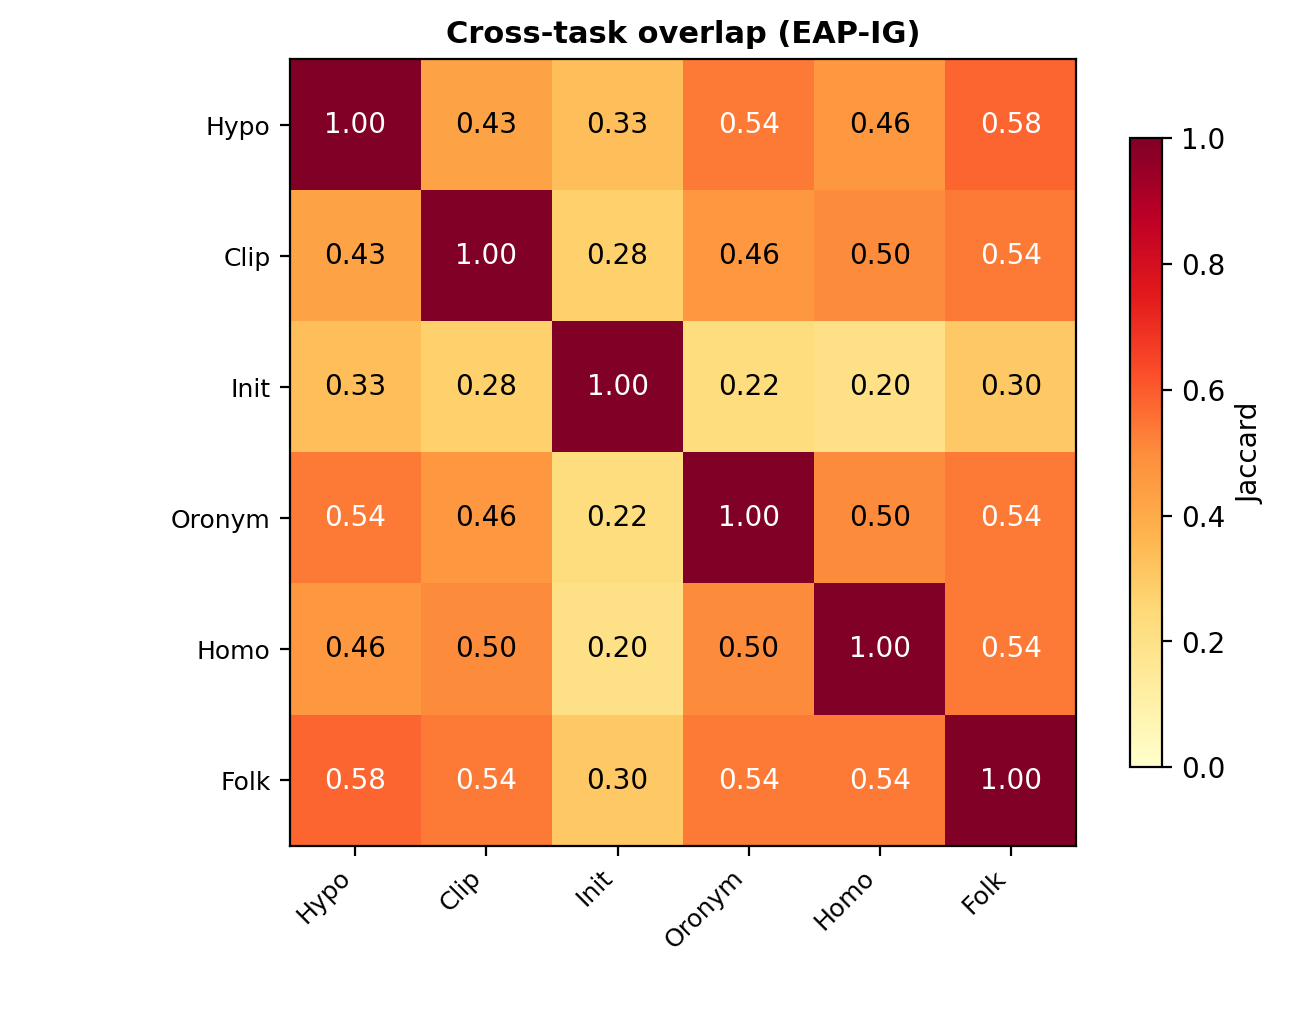
\includegraphics[width=\textwidth]{figures/cross_task_heatmap.png}
\end{center}
{\scriptsize Jaccard similarity of top-30 heads between each task pair. Initialism is most distinct ($J \leq 0.30$). Hypo--Folk and Orny--Folk highest (0.58).}
\end{column}

\begin{column}{0.48\textwidth}
\begin{center}
\textbf{Jaccard MDS}\\[4pt]
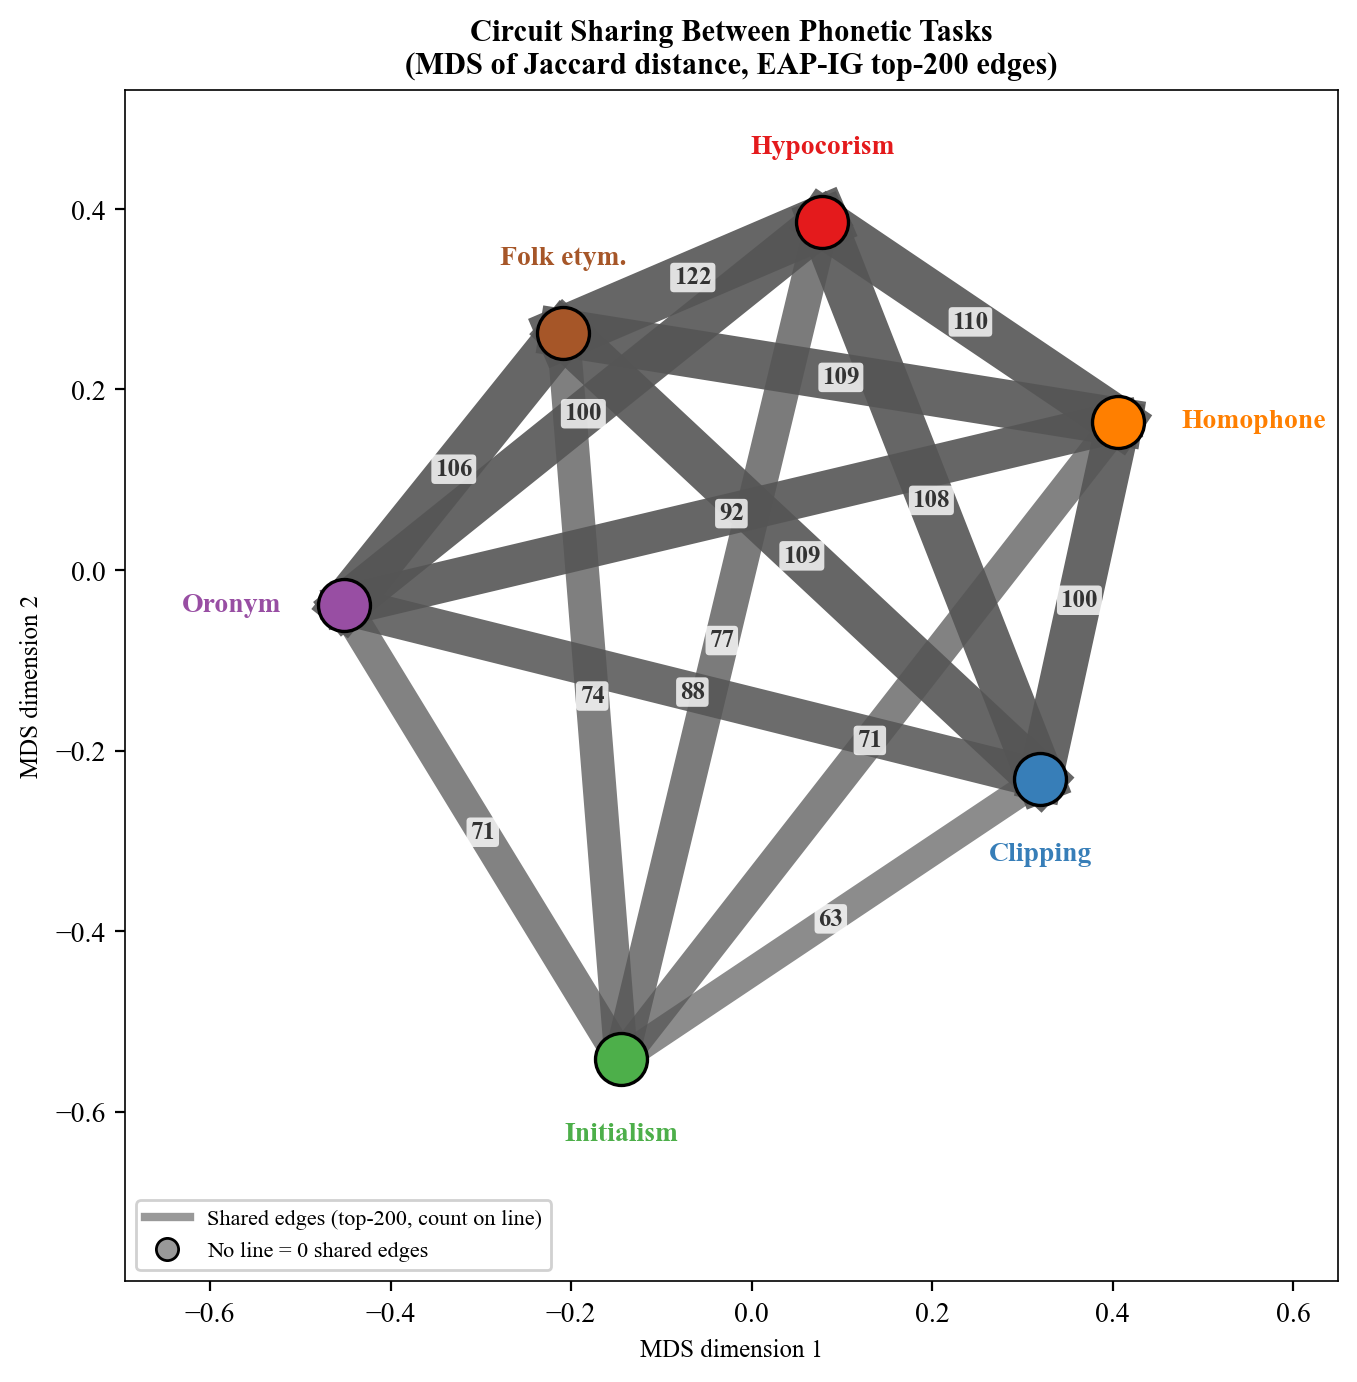
\includegraphics[width=\textwidth]{../results/plots/jaccard_mds.png}
\end{center}
{\scriptsize MDS embedding of circuit Jaccard distances. Tasks cluster by computational type. Initialism is an outlier; oronym, hypocorism, and folk etymology cluster together.}
\end{column}
\end{columns}

\vspace{0.3em}
{\small Shared backbone (H1) confirmed: most tasks share $\geq$40\% of top heads. Distinct specialists (H2): initialism recruits unique heads.}
\end{frame}

% =============================================
% HEAD USAGE HEATMAP
% =============================================
\begin{frame}{The backbone: which heads are shared across tasks?}

\begin{center}
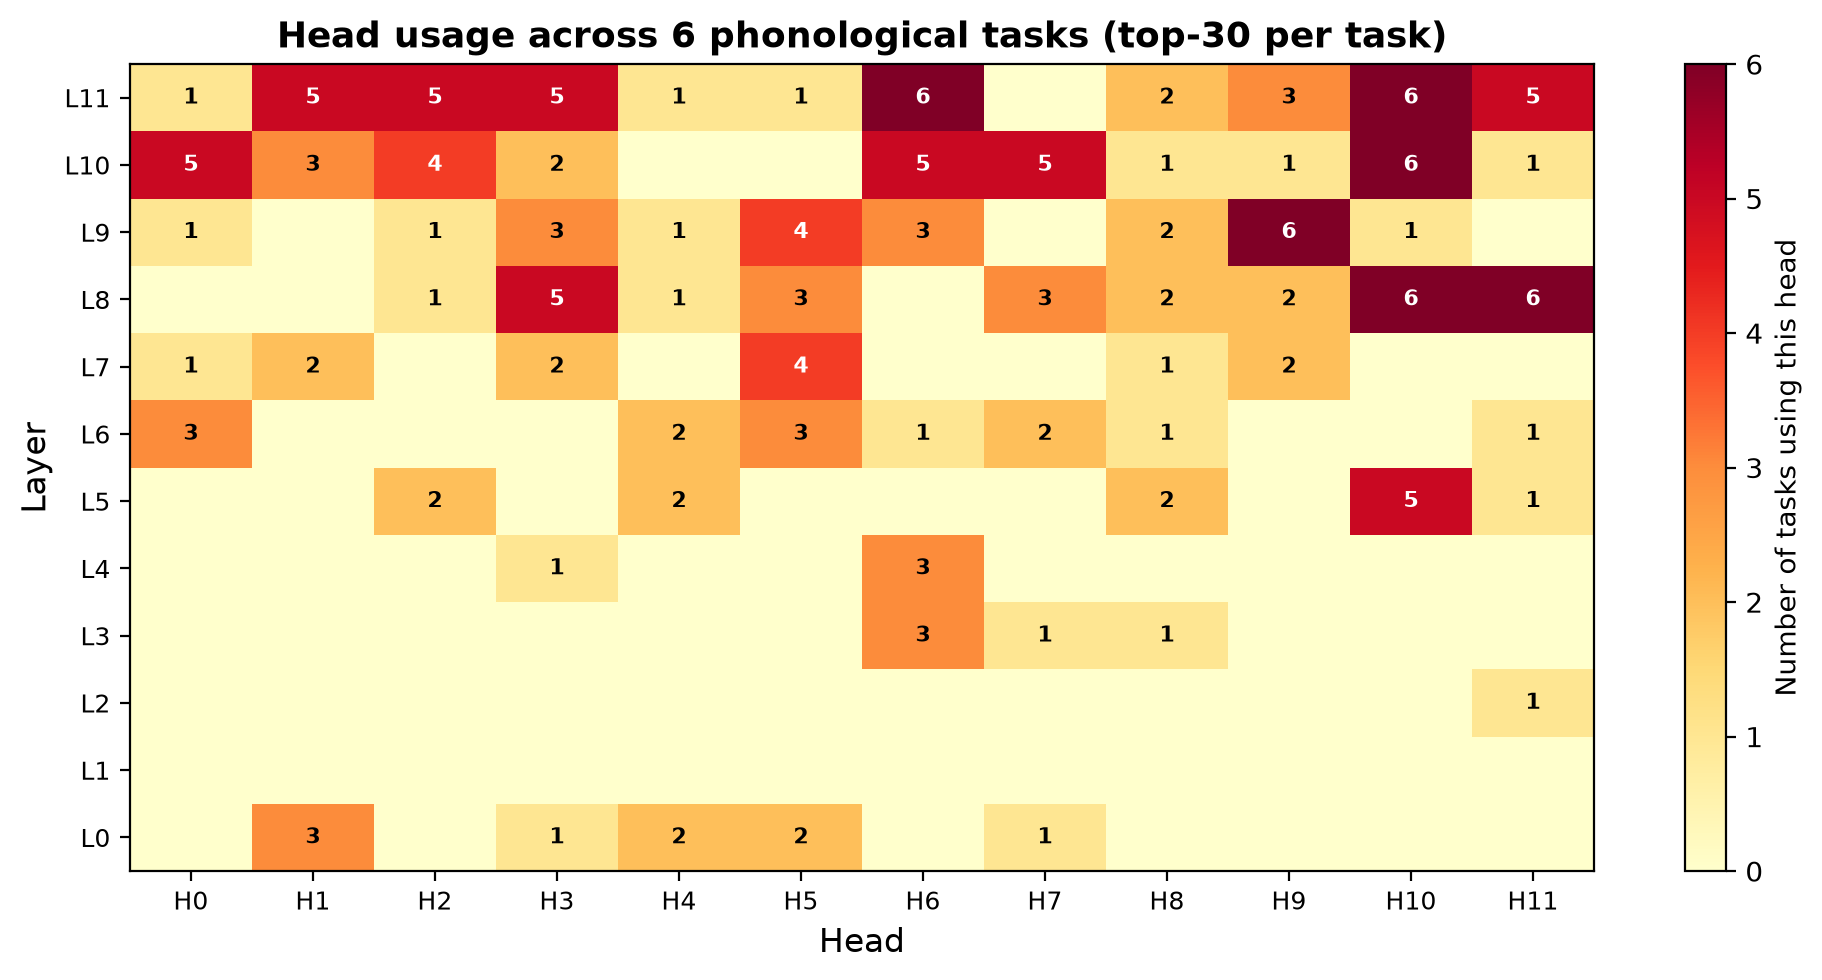
\includegraphics[width=0.9\textwidth]{figures/head_usage_heatmap.png}
\end{center}

\vspace{0.3em}
{\small 6 heads appear in all 6 tasks (L8.H10, L8.H11, L9.H9, L10.H10, L11.H6, L11.H10) --- all in L8--11. 15 heads in 5+ tasks, 18 in 4+. Initialism has 11 unique heads (most of any task). The backbone is real and concentrated in late layers.}
\end{frame}

% =============================================
% SUB-CIRCUIT CONTAINMENT
% =============================================
\begin{frame}{Sub-circuit containment}

\begin{columns}[T]
\begin{column}{0.52\textwidth}
\begin{center}
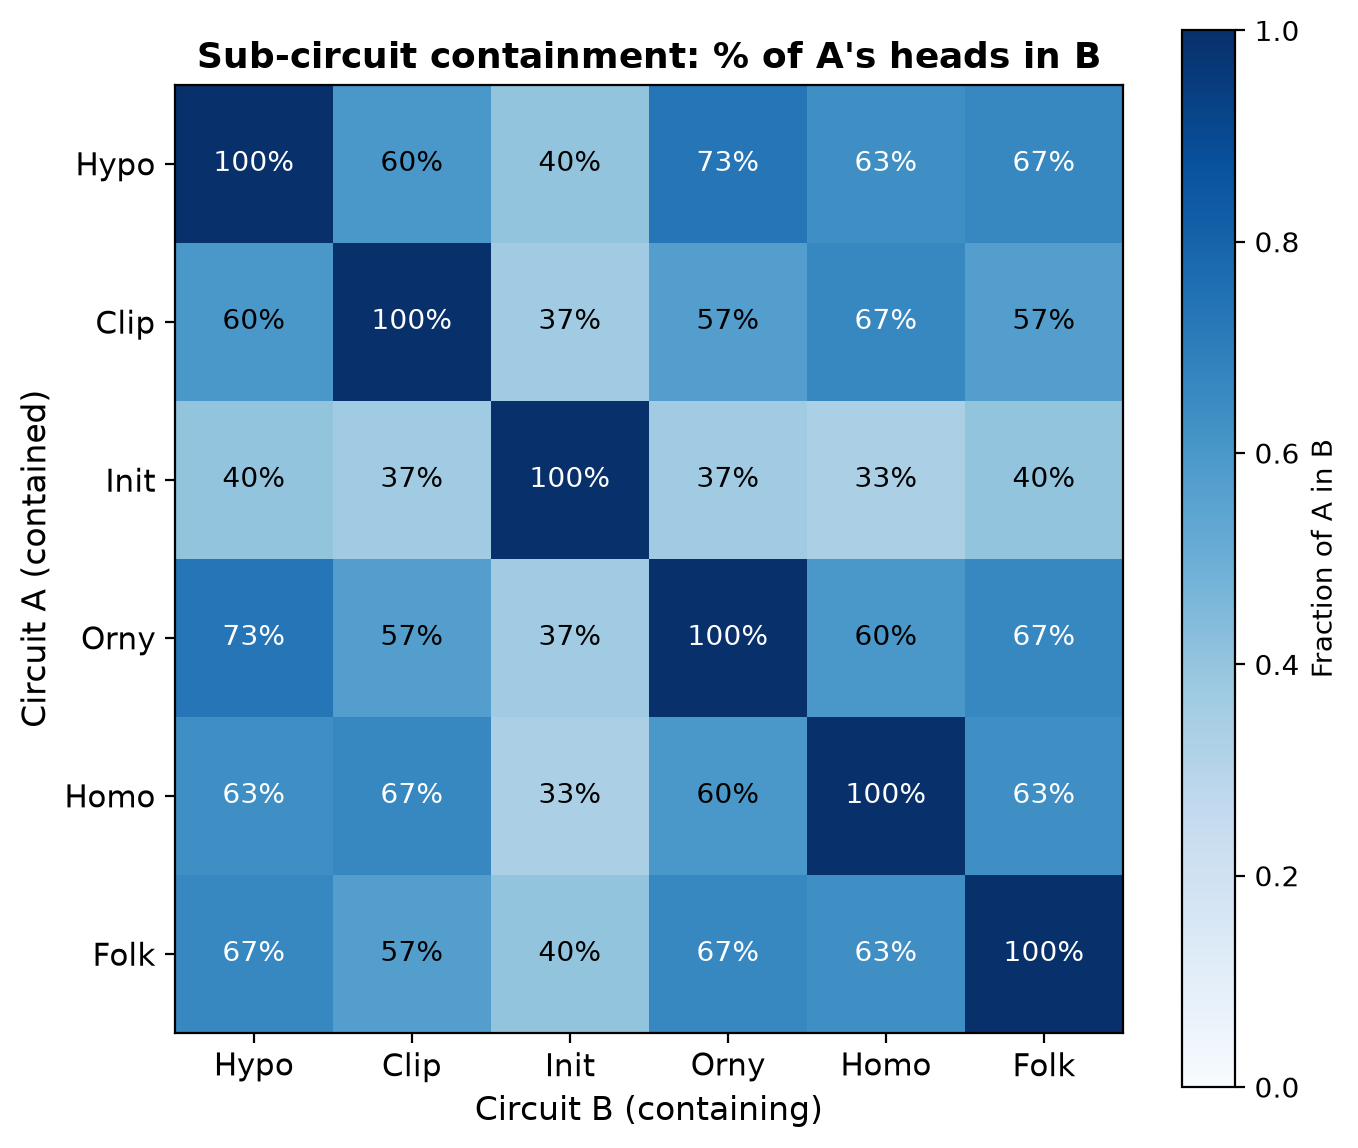
\includegraphics[width=\textwidth]{figures/containment_matrix.png}
\end{center}
\end{column}

\begin{column}{0.45\textwidth}
\vspace{1em}
Read as: ``\% of row circuit's heads found in column circuit.''

\vspace{0.5em}
\textbf{Key findings:}
\begin{itemize}
  \item Hypo $\leftrightarrow$ Orny: mutual 73\% containment
  \item Folk is 67\% contained in both Hypo and Orny
  \item Init is only 33--40\% contained in anything --- the most distinct circuit
  \item Homo--Clip: 67\% mutual containment
\end{itemize}

\vspace{0.5em}
{\small Not a simple hierarchy --- circuits overlap symmetrically, suggesting a shared computational core with task-specific extensions.}
\end{column}
\end{columns}
\end{frame}

% =============================================
% LAYER-RESOLVED JACCARD
% =============================================
\begin{frame}{Where overlap happens: layer-resolved Jaccard}

\begin{center}
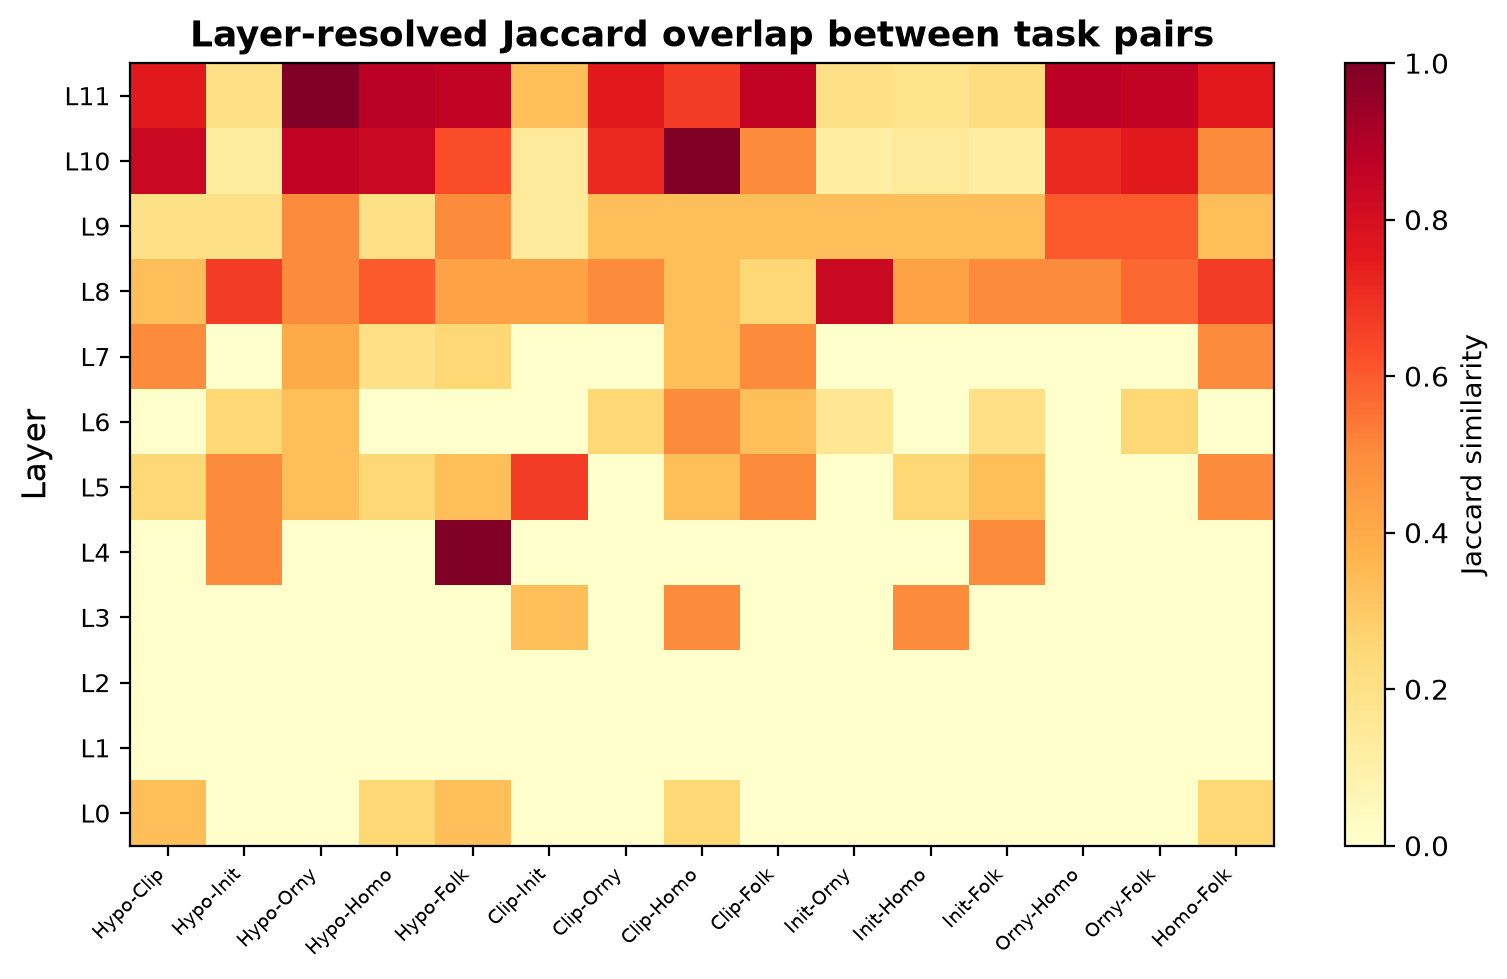
\includegraphics[width=0.85\textwidth]{figures/layer_resolved_jaccard.png}
\end{center}

\vspace{0.3em}
{\small Layers 0--7: mean Jaccard 0.10--0.28 (task-specific). Layers 8--11: mean Jaccard 0.35--0.63 (shared backbone). The backbone is not just ``the same layers'' --- it is literally the same heads within those layers.}
\end{frame}

% =============================================
% FAITHFULNESS CURVES
% =============================================
\begin{frame}{Faithfulness: circuits recover full-model performance}

\begin{center}
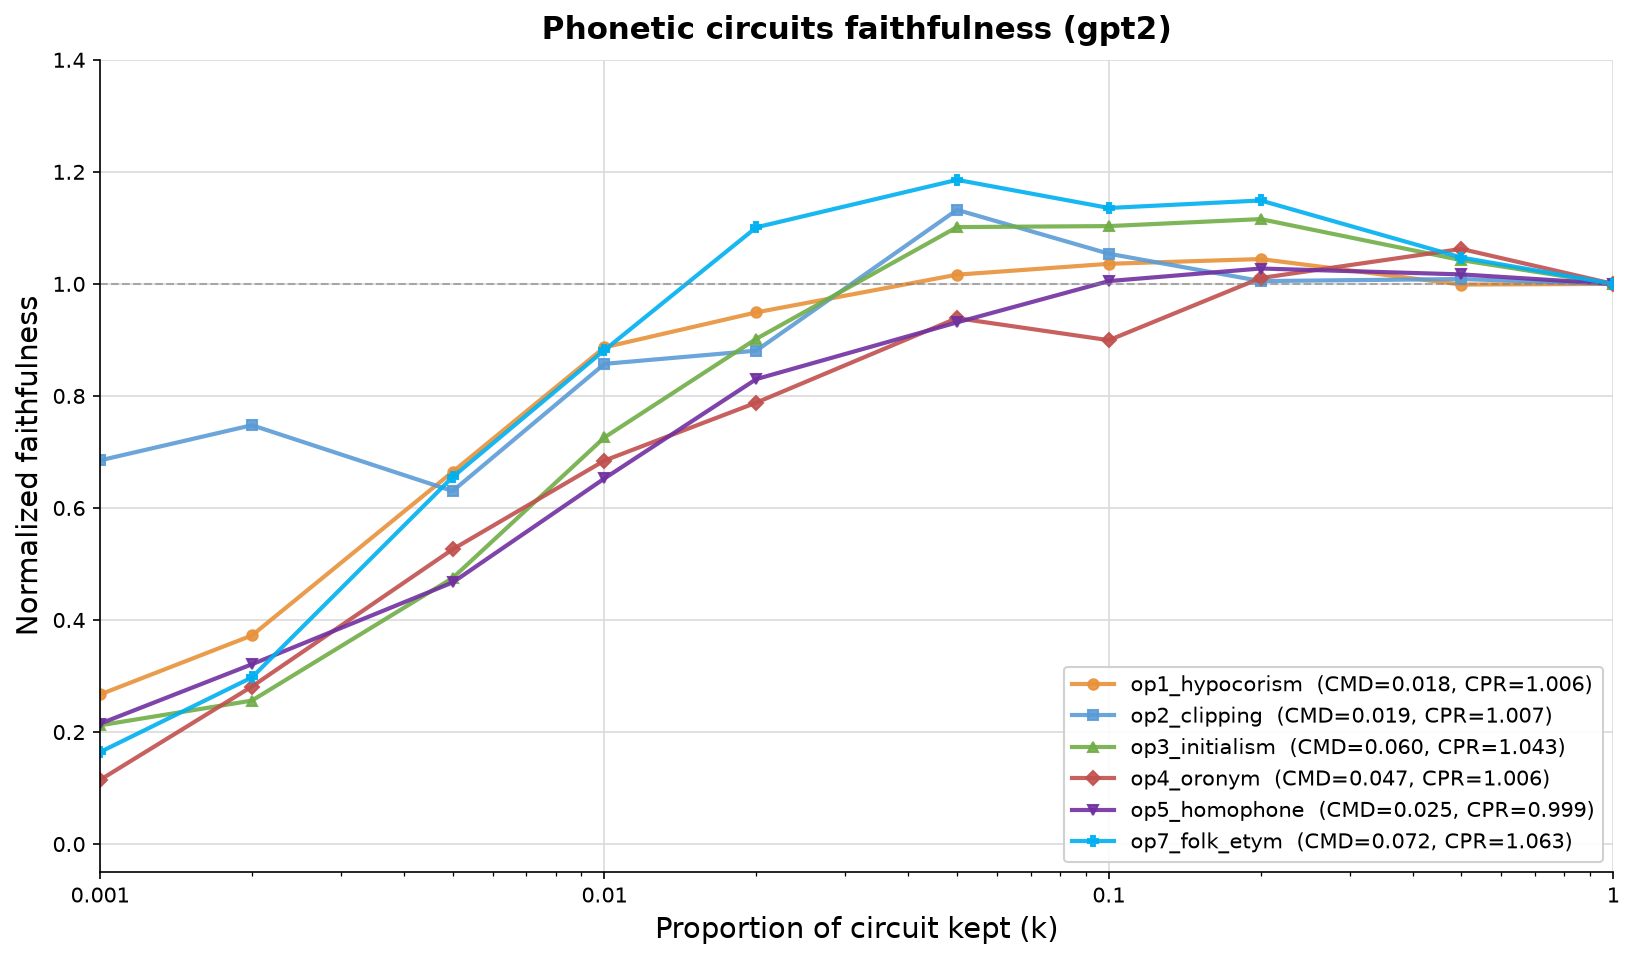
\includegraphics[width=0.7\textwidth]{../results/plots/overlay_gpt2.png}
\end{center}

\vspace{-0.3em}
{\small All six tasks reach $>$95\% of full-model performance with $<$5\% of edges.

Sparse, faithful circuits exist for every phonological operation in GPT-2.}
\end{frame}

% =============================================
% CAUSAL INFERENCE SUB-SECTION
% =============================================
\begin{frame}{Causal inference: validating circuits with three methods}

\begin{center}
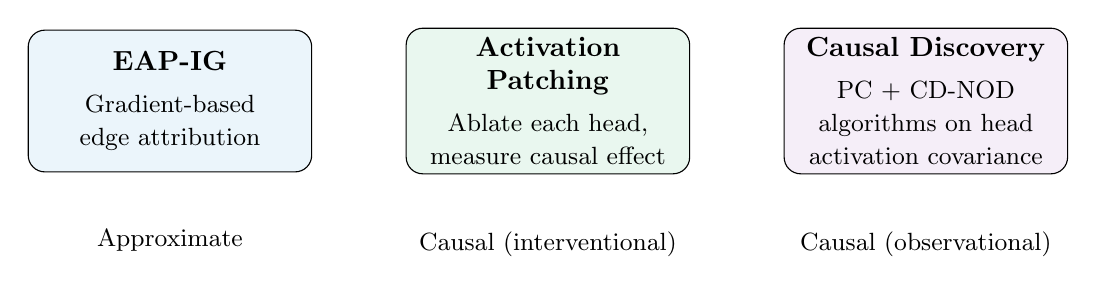
\begin{tikzpicture}[
  method/.style={draw, rounded corners=6pt, minimum height=1.8cm, minimum width=3.6cm,
               align=center, font=\normalsize},
]
  \node[method, fill=accent!10] (eap) at (0, 0) {
    \textbf{EAP-IG}\\[3pt]
    {\small Gradient-based}\\
    {\small edge attribution}
  };

  \node[method, fill=circuit!10] (ap) at (4.8, 0) {
    \textbf{Activation}\\
    \textbf{Patching}\\[3pt]
    {\small Ablate each head,}\\
    {\small measure causal effect}
  };

  \node[method, fill=fusion!10] (cd) at (9.6, 0) {
    \textbf{Causal Discovery}\\[3pt]
    {\small PC + CD-NOD}\\
    {\small algorithms on head}\\
    {\small activation covariance}
  };

  \node[font=\small, below=0.6cm of eap] {Approximate};
  \node[font=\small, below=0.6cm of ap] {Causal (interventional)};
  \node[font=\small, below=0.6cm of cd] {Causal (observational)};
\end{tikzpicture}
\end{center}

\vspace{0.5em}
If all three converge on the same heads $\to$ strong evidence the circuit is real, not an artifact of any single method.
\end{frame}

% =============================================
% EAP-IG vs ACT PATCHING
% =============================================
\begin{frame}{EAP-IG vs activation patching: head-by-head}

\begin{center}
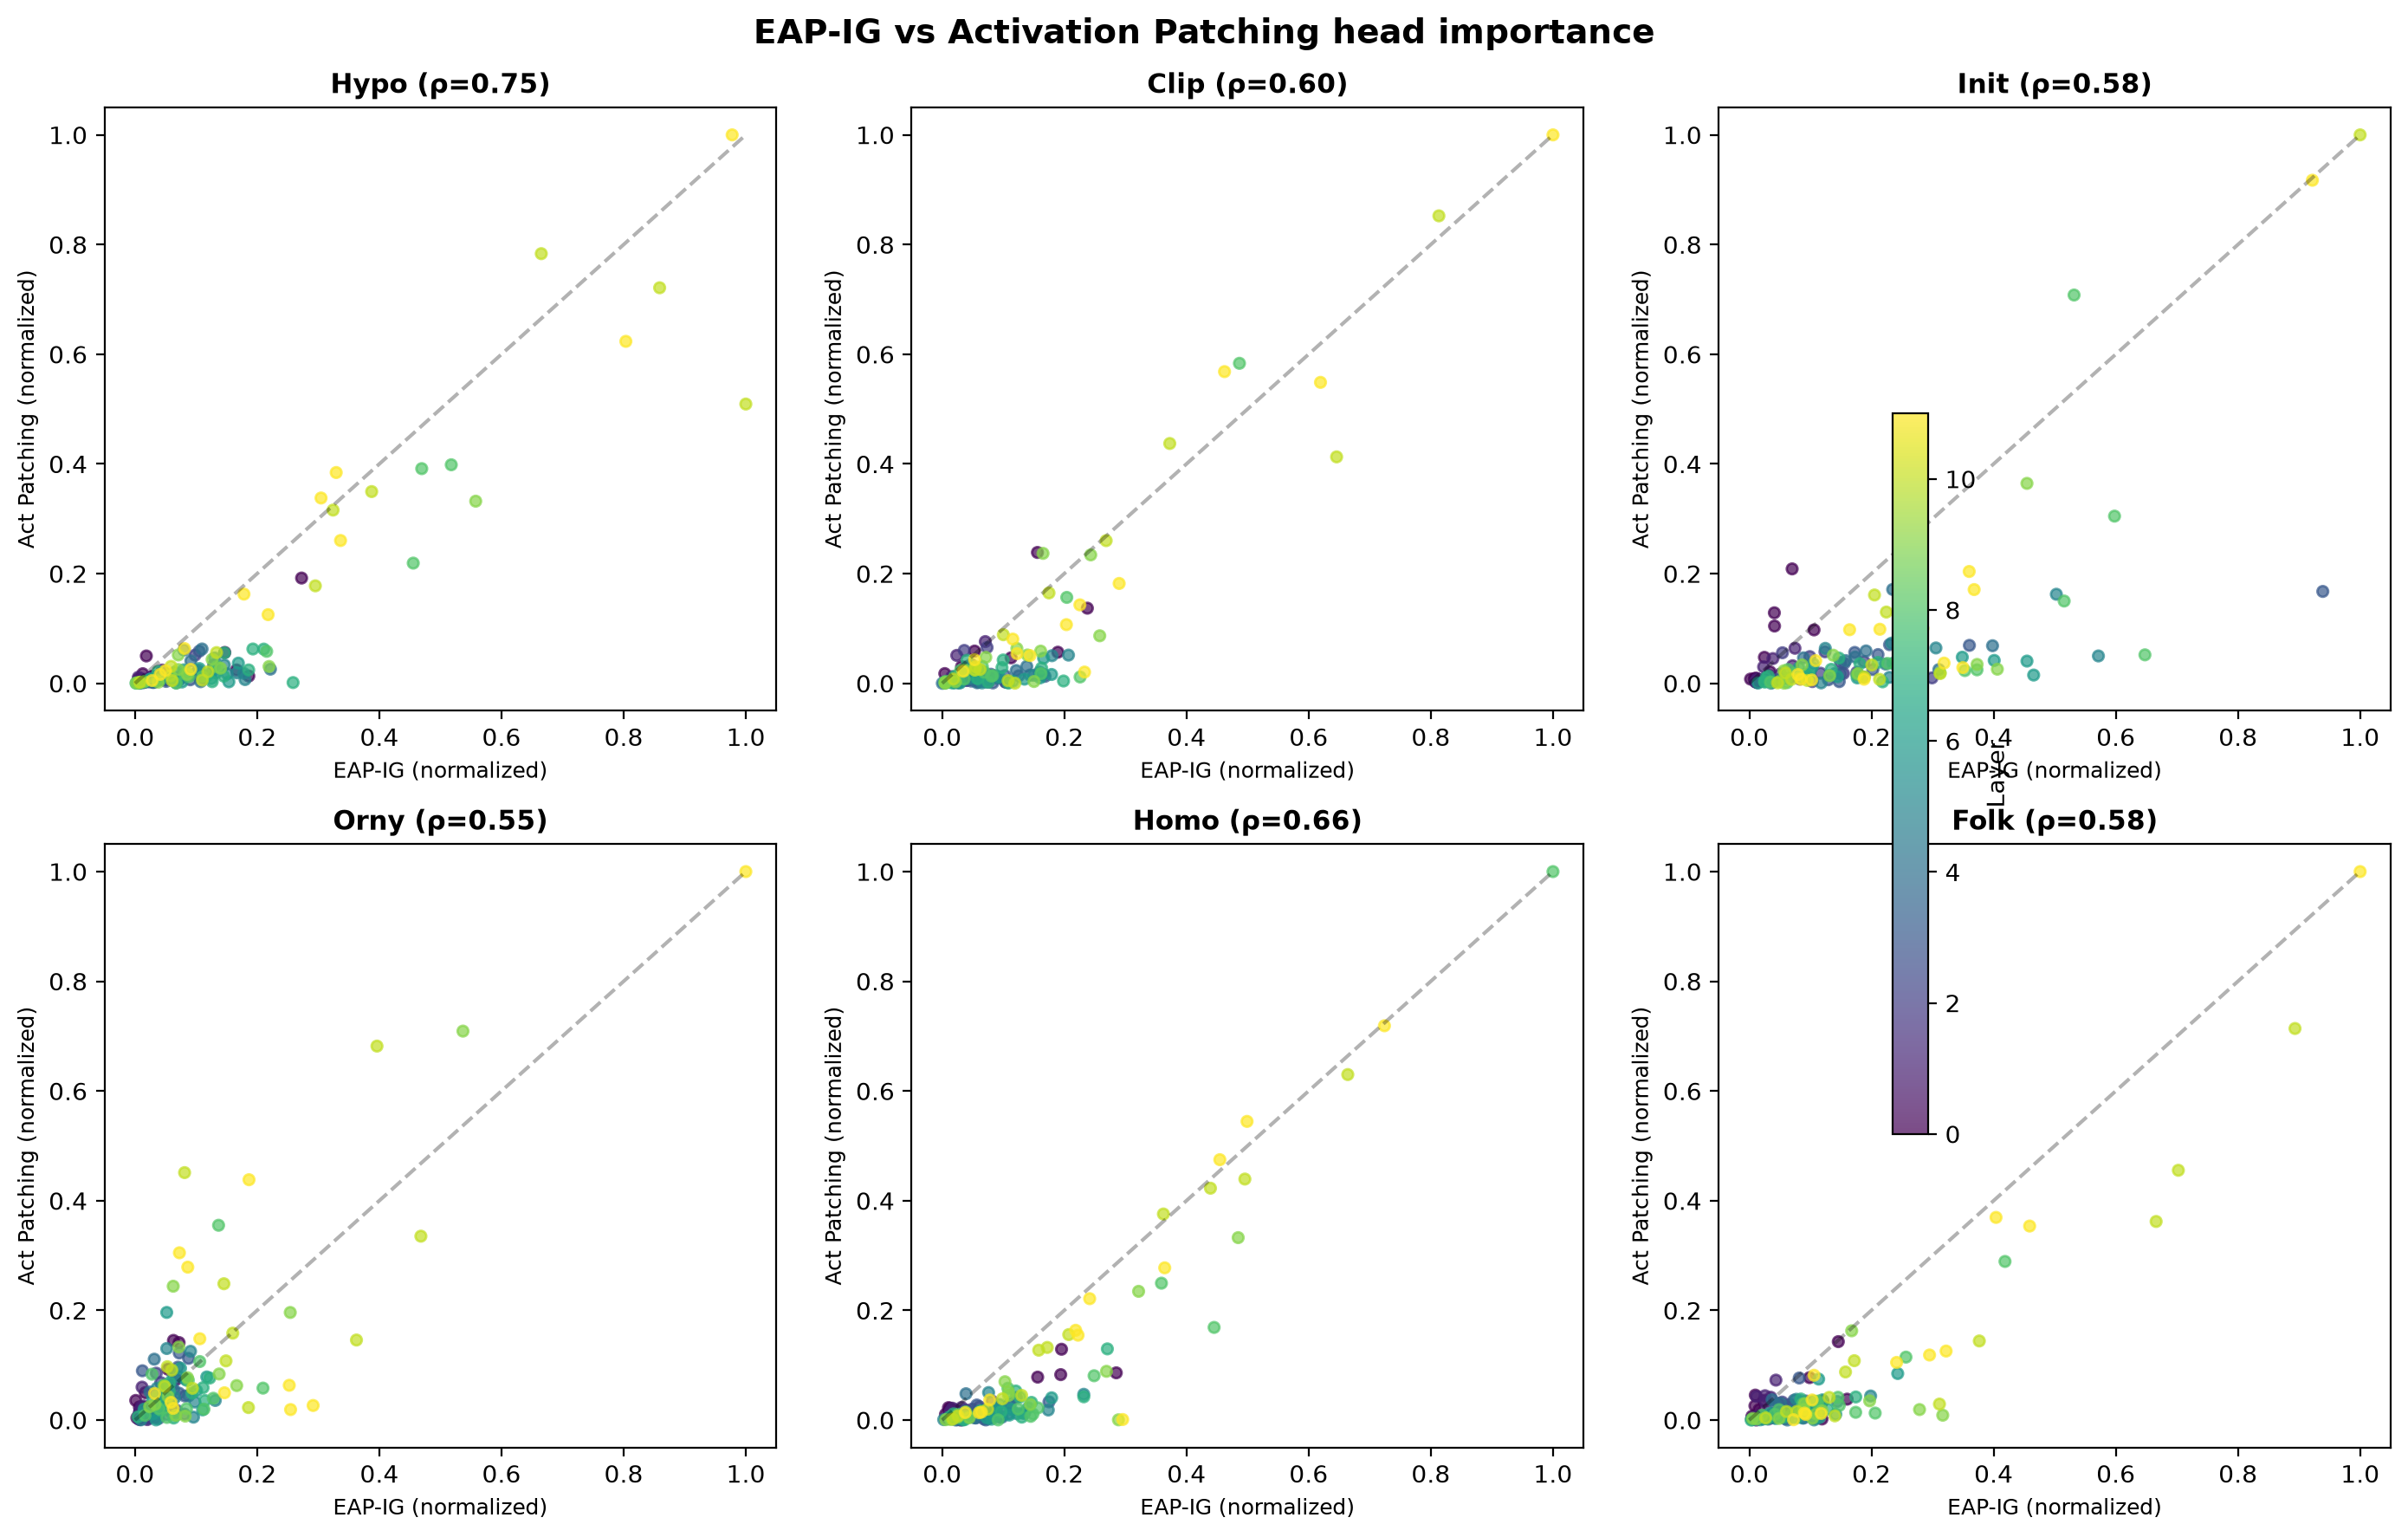
\includegraphics[width=0.85\textwidth]{figures/eap_vs_actpatch.png}
\end{center}

\vspace{0.3em}
{\small Spearman $\rho$ = 0.55--0.75 across all tasks ($p < 10^{-12}$). Color = layer. Top-30 head overlap: 13--23 of 30. Late-layer heads (yellow/green) cluster in the high-importance corner --- the backbone heads are validated by both methods.}
\end{frame}

% =============================================
% 3-METHOD AGREEMENT
% =============================================
\begin{frame}{Method agreement across all three}

\begin{columns}[T]
\begin{column}{0.48\textwidth}
\begin{center}
\textbf{Head-level agreement}\\[4pt]
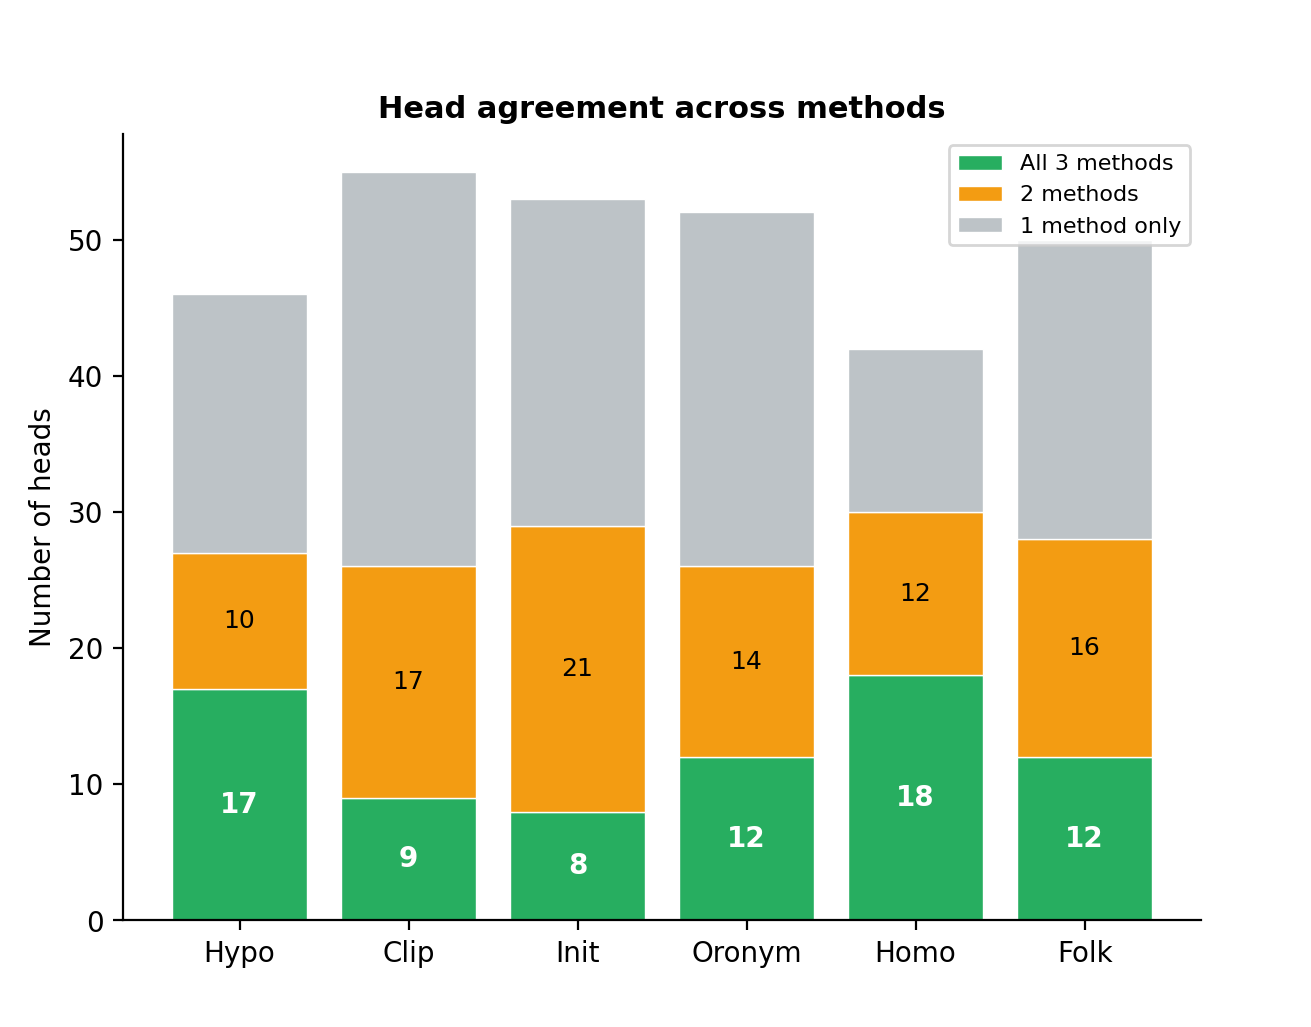
\includegraphics[width=\textwidth]{figures/head_agreement_stacked.png}
\end{center}
{\scriptsize Stacked bars: green = all 3 methods agree, orange = 2 of 3, gray = 1 only. Homophone has highest triple agreement (18 heads).}
\end{column}

\begin{column}{0.48\textwidth}
\begin{center}
\textbf{Where do all 3 methods agree?}\\[4pt]
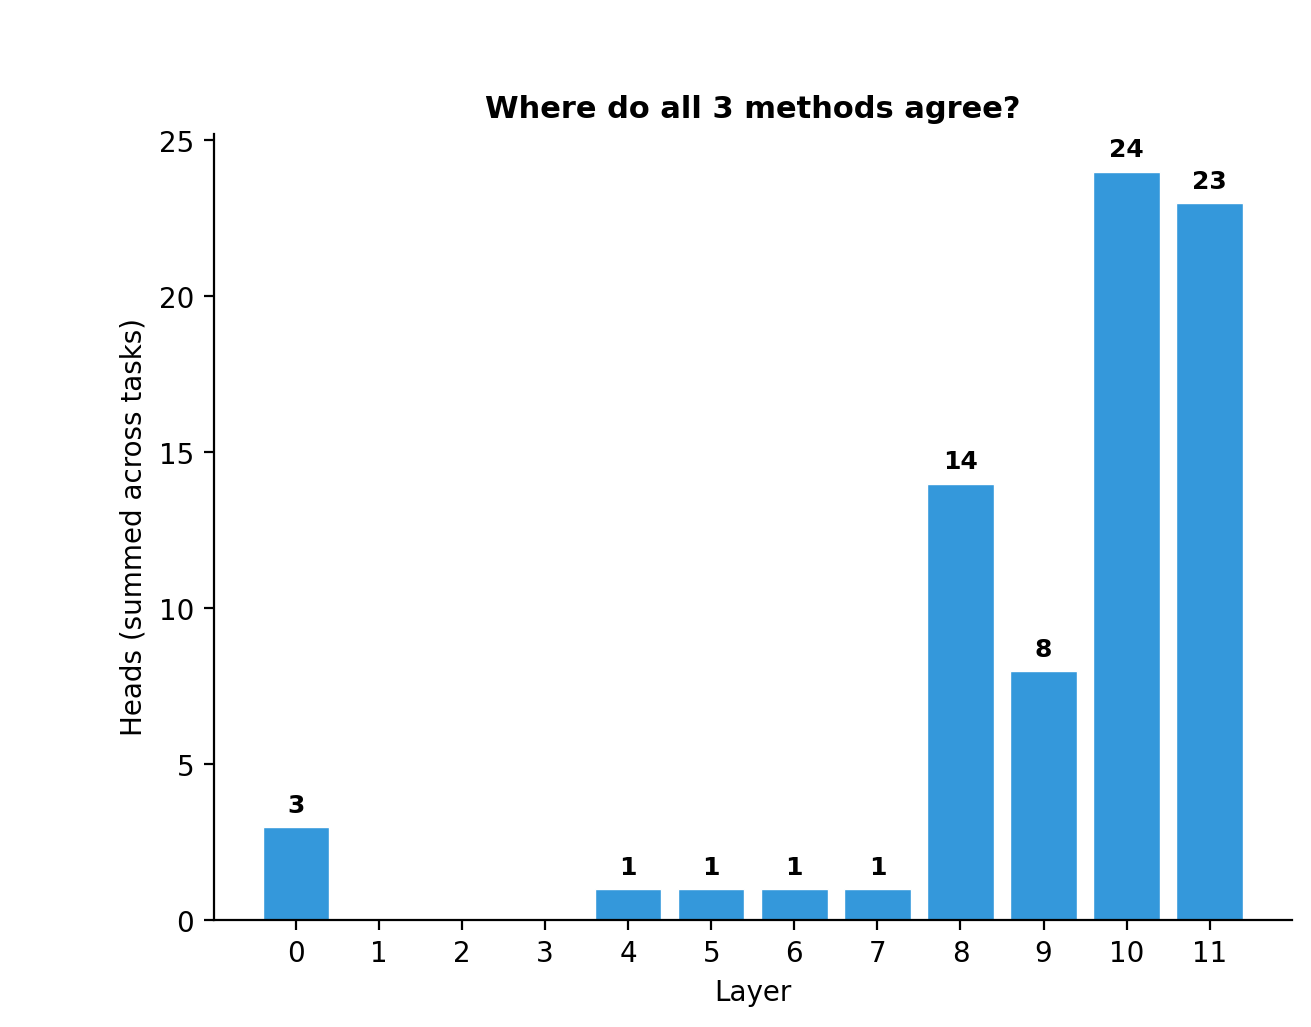
\includegraphics[width=\textwidth]{figures/layer_distribution.png}
\end{center}
{\scriptsize 91\% of triple-agreed heads are in layers 8--11. Layer 10 alone accounts for 24 head-task pairs.}
\end{column}
\end{columns}

\vspace{0.3em}
{\small Methods agree well on \textbf{which heads} matter (8--18 triple-agreed per task). Edge-level agreement is lower --- expected, since edges are a finer-grained unit.}
\end{frame}

% =============================================
% CAUSAL DISCOVERY: DO THE ALGORITHMS AGREE?
% =============================================
\hypertarget{sl:causaldiscovery}{}
\begin{frame}{Causal discovery: do the algorithms agree?}

\begin{columns}[T]
\begin{column}{0.45\textwidth}
\textbf{Setup:}
\begin{itemize}
  \item Top-30 heads by activation variance (clean vs.\ corrupted)
  \item Per-head activation norms at last token
  \item Two algorithms run independently:
  \begin{itemize}
    \item \textbf{PC}: conditional independence only
    \item \textbf{CD-NOD} (\href{https://www.jmlr.org/papers/v21/19-232.html}{Huang et al., 2020}): exploits clean/corrupted distribution shift to orient edges
  \end{itemize}
\end{itemize}

\vspace{0.3em}
\textbf{Result: 96--100\% agreement.}\\
CD-NOD's extra signal adds almost nothing --- conditional independence alone finds the graph.
\end{column}

\begin{column}{0.53\textwidth}
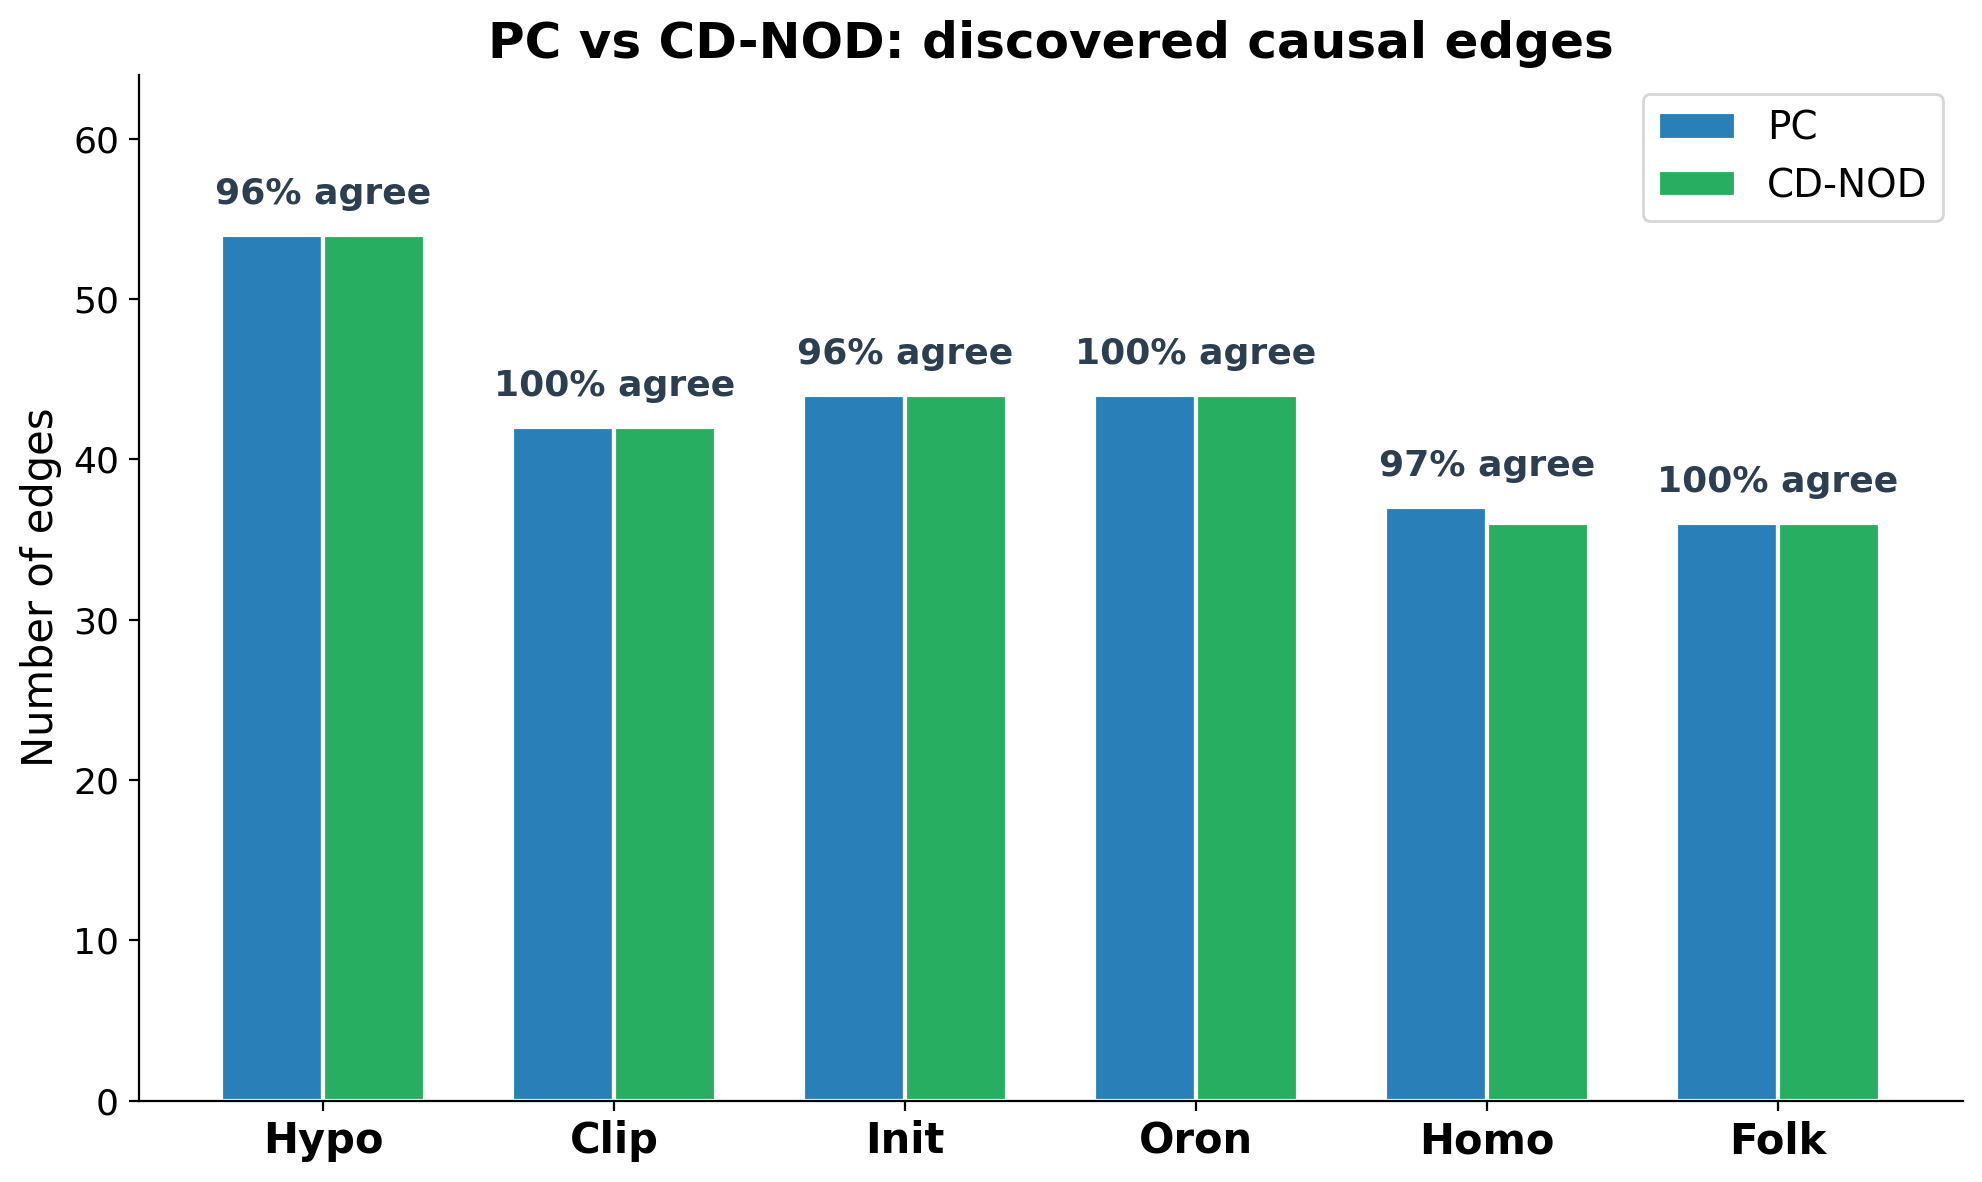
\includegraphics[width=\textwidth]{figures/causal_discovery_agreement.png}
\end{column}
\end{columns}
\end{frame}

% =============================================
% CAUSAL DISCOVERY: HUB HEADS
% =============================================
\begin{frame}{Causal discovery: hub heads across tasks}

\begin{columns}[T]
\begin{column}{0.40\textwidth}
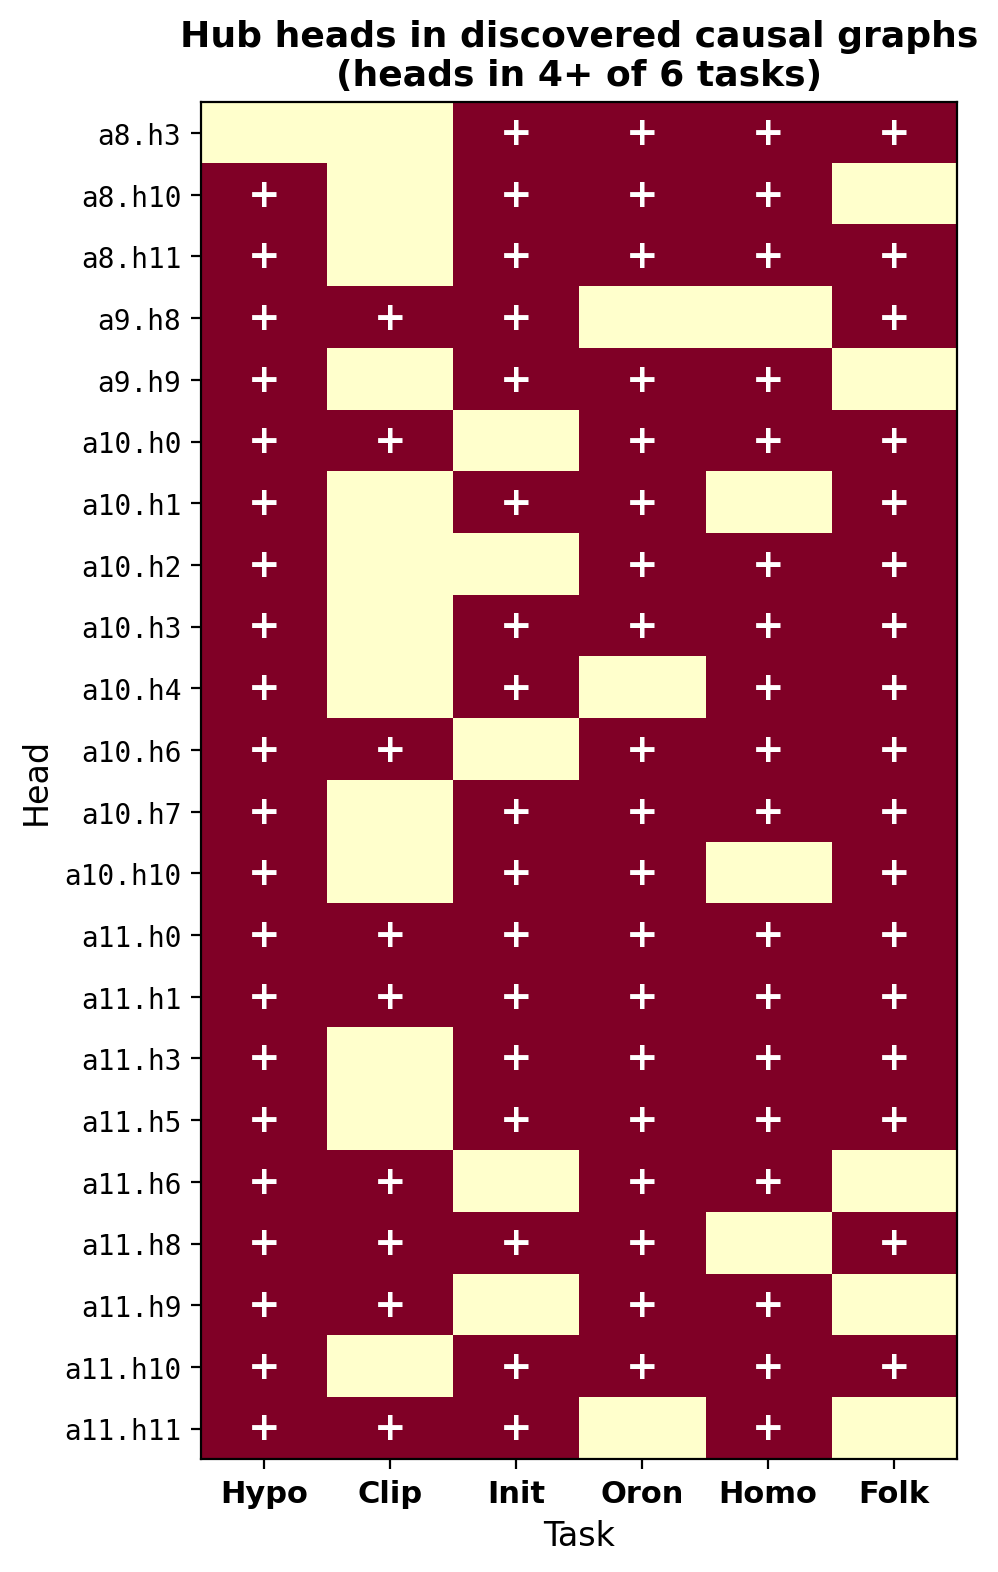
\includegraphics[width=\textwidth,height=0.78\textheight,keepaspectratio]{figures/causal_discovery_hub_heads.png}
\end{column}

\begin{column}{0.53\textwidth}
\textbf{Universal hubs} (all 6 tasks):\\[0.2em]
\texttt{a11.h0} (sink) and \texttt{a11.h1} (source) --- same heads EAP identifies as circuit-critical

\vspace{0.3em}
\textbf{Layer distribution:}\\
21/22 hub heads are in layers 8--11. Early heads appear only in task-specific edges, never as hubs.

\vspace{0.3em}
\textbf{Recurring edge:}\\
\texttt{a8.h11} $\to$ \texttt{a10.h7} in 3/6 tasks

\vspace{0.3em}
\textbf{Source vs.\ sink structure:}\\
\small
\begin{tabular}{lll}
Hypo: & \texttt{a10.h10} $\to$ 8 heads & 10 $\to$ \texttt{a10.h0} \\
Clip: & \texttt{a11.h6} $\to$ 8 heads & 8 $\to$ \texttt{a7.h0} \\
Oron: & \texttt{a11.h8} $\to$ 6 heads & 10 $\to$ \texttt{a10.h7} \\
\end{tabular}

\vspace{0.3em}
\textbf{Implication:} the causal graph we hypothesized aligns with what the algorithms discover independently.
\end{column}
\end{columns}
\end{frame}

% =============================================
% CAUSAL VALIDATION SUMMARY
% =============================================
\begin{frame}{Circuit validation summary}

\textbf{Three independent methods converge:}
\begin{itemize}
  \item \textbf{EAP-IG} (gradient-based) finds sparse, faithful circuits for all 6 tasks
  \item \textbf{Activation patching} (interventional) validates the same head rankings
  \item \textbf{Causal discovery} (observational) independently recovers the same hub heads and layer structure
\end{itemize}

\vspace{0.5em}
\textbf{Key findings:}
\begin{itemize}
  \item 8--18 heads per task where all 3 methods agree
  \item 91\% of triple-agreed heads in layers 8--11
  \item Universal hub heads (\texttt{a11.h0}, \texttt{a11.h1}) appear in all tasks across all methods
  \item PC and CD-NOD agree 96--100\% --- the causal structure is robust
\end{itemize}

\vspace{0.5em}
{\small \textbf{Open question:} We currently assume the causal graph (name $\to$ shorten $\to$ fuse $\to$ output) and test alignment. Can we instead \emph{discover} the model's causal structure from activation data? This would let the model tell us what operations it performs, rather than confirming or denying our hypotheses.}
\end{frame}

% =============================================
% PART 6 DIVIDER — CAUSAL VARIABLE LOCALIZATION
% =============================================
\begin{frame}[plain,noframenumbering]
\begin{center}
\vfill
  {\setlength{\fboxrule}{2.5pt}\fcolorbox{black}{white}{\parbox{0.7\textwidth}{\centering\vspace{0.8em}
    {\Large\bfseries Part 6: Causal Variable Localization}\\[4pt]
    {\normalsize What flows along the edges?}
  \vspace{0.8em}}}}
\vfill
\end{center}
\end{frame}

% =============================================
% CVL MOTIVATION
% =============================================
\begin{frame}{From circuits to causal variables}
\hypertarget{sl:cvl}{}

Circuit localization tells us \textbf{which} heads matter. But not \textbf{what} they communicate.

\vspace{0.8em}
\begin{center}
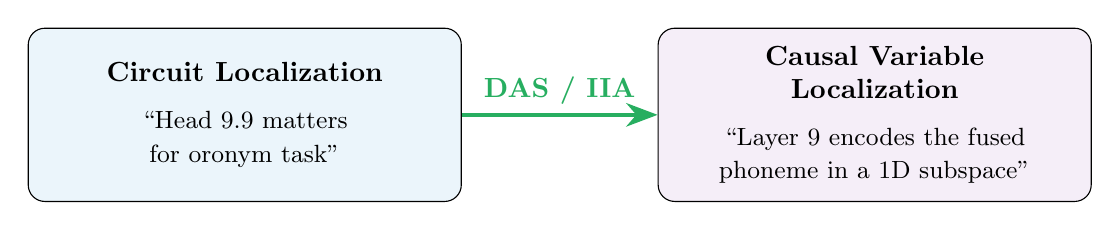
\begin{tikzpicture}[
  box/.style={draw, rounded corners=6pt, minimum height=2.2cm, minimum width=5.5cm,
              align=center, font=\normalsize},
  arr/.style={-{Stealth[length=4mm]}, very thick}
]
  \node[box, fill=accent!10] (cl) at (0, 0) {
    \textbf{Circuit Localization}\\[5pt]
    {\small ``Head 9.9 matters}\\
    {\small for oronym task''}
  };

  \node[box, fill=fusion!10] (cvl) at (8, 0) {
    \textbf{Causal Variable}\\
    \textbf{Localization}\\[5pt]
    {\small ``Layer 9 encodes the fused}\\
    {\small phoneme in a 1D subspace''}
  };

  \draw[arr, circuit] (cl) -- (cvl)
    node[midway, above, font=\normalsize\bfseries] {DAS / IIA};
\end{tikzpicture}
\end{center}

\vspace{0.8em}
\textbf{Method:} \href{https://arxiv.org/abs/2303.02536}{Distributed Alignment Search} (DAS; Geiger et al., 2024) --- find a linear subspace in the residual stream at each layer that encodes a specific causal variable (e.g., the target phoneme).

\vspace{0.3em}
\textbf{Metric:} Interchange Intervention Accuracy (IIA) --- swap the subspace between two inputs and check if the output changes as predicted.
\end{frame}

% =============================================
% CAUSAL VARIABLES
% =============================================
\begin{frame}{Causal variables for phonological tasks}

\small
Each operation implies a different causal variable:

\vspace{0.5em}
\begin{center}
\renewcommand{\arraystretch}{1.2}
\begin{tabular}{lll}
\toprule
\textbf{Op} & \textbf{Task} & \textbf{Causal variable} \\
\midrule
1 & Hypocorism & Nickname identity (Robert $\to$ Bob) \\
2 & Clipping & First-syllable boundary position \\
3 & Initialism & Letter $\to$ phoneme name mapping \\
\rowcolor{fusion!8}
4 & \textbf{Oronym} & \textbf{Fused phoneme string (cross-boundary)} \\
5 & Homophone & Phoneme identity across spellings \\
7 & Folk etymology & Decomposition boundaries \\
\bottomrule
\end{tabular}
\end{center}

\vspace{0.5em}
\textbf{Key question:} does layer 9 encode the \emph{fused phoneme string} for oronyms in a linear subspace?

If IIA is high on the oronym circuit heads but low elsewhere $\Rightarrow$ the circuit is \textbf{causally} responsible, not just correlated.
\end{frame}

% =============================================
% DAS RESULTS (PLACEHOLDER)
% =============================================
\begin{frame}{DAS results: IIA by layer}
\hypertarget{sl:dasresults}{}

\begin{center}
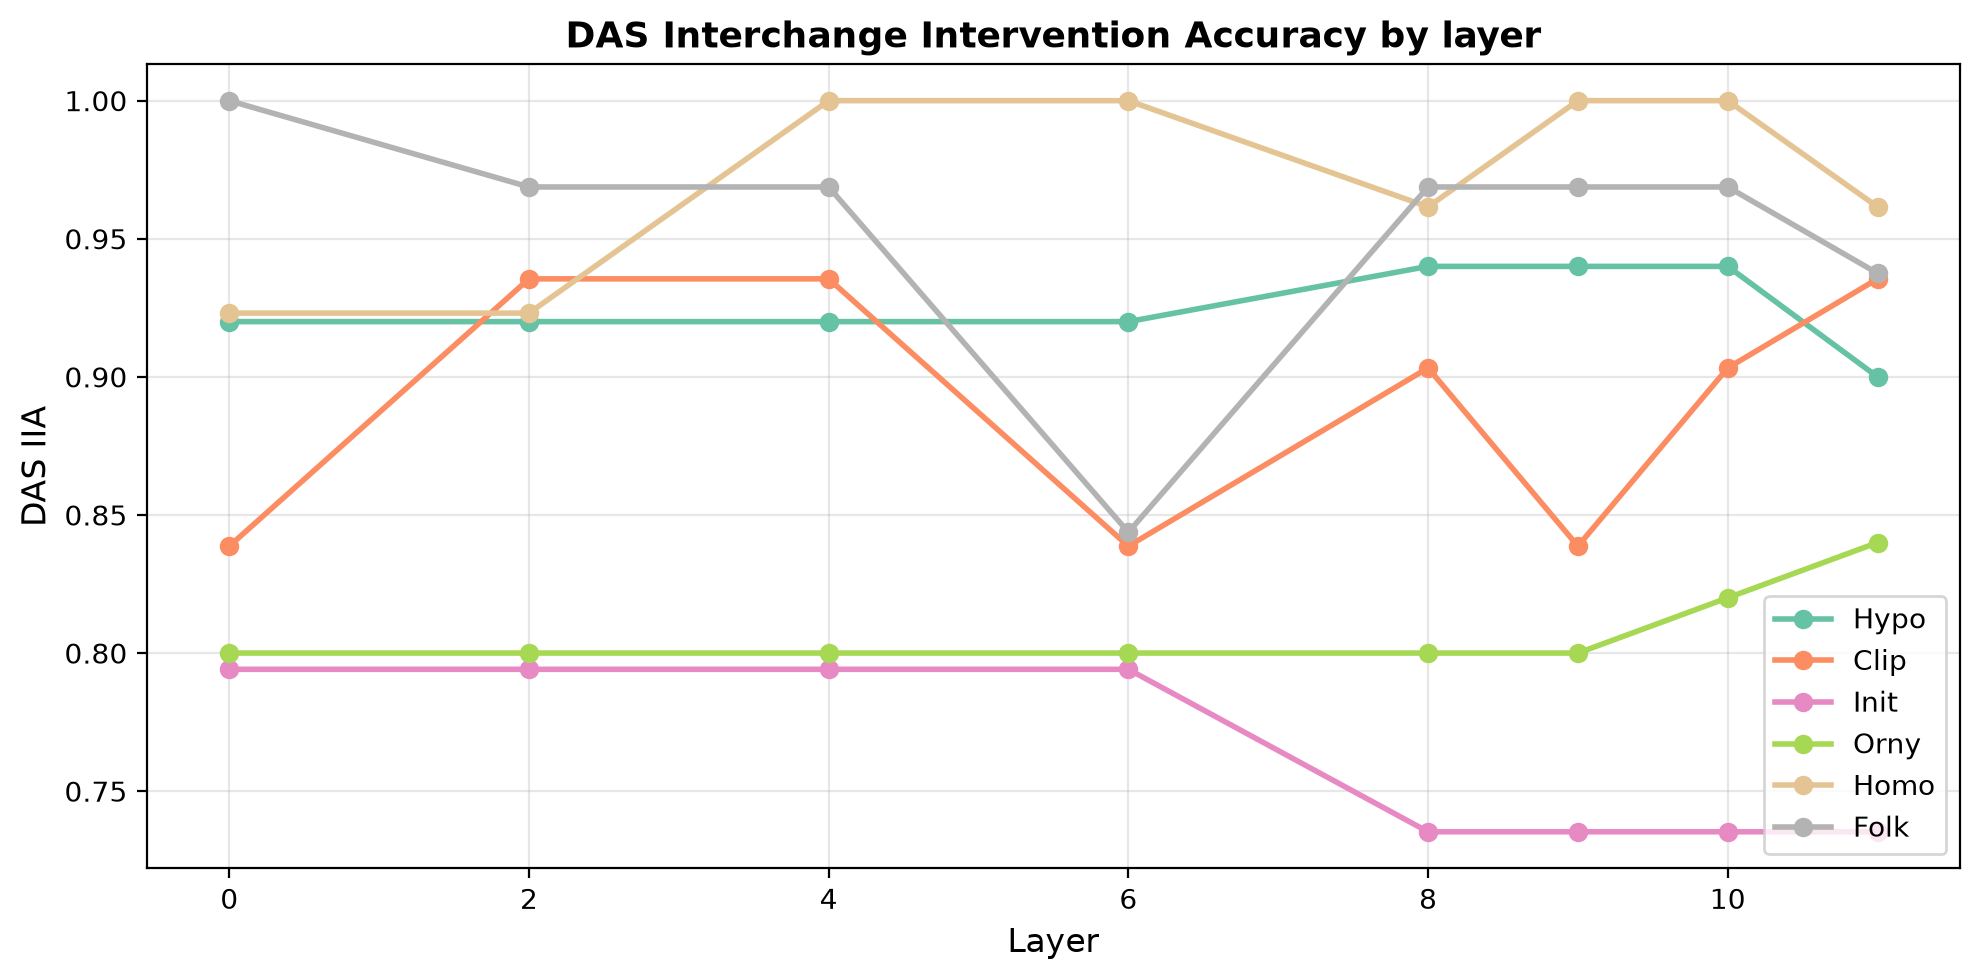
\includegraphics[width=0.85\textwidth]{figures/das_iia_by_layer.png}
\end{center}

\vspace{0.3em}
{\small Rank-1 DAS probes trained per layer per task. Homophone and folk etymology reach IIA = 1.0 (perfect causal alignment). Hypocorism peaks at L8 (0.94). Initialism is hardest (0.79 max). Most tasks have flat IIA curves --- causal variables are accessible at multiple layers, not strongly localized.}
\end{frame}

\begin{frame}{DAS results: what the numbers mean}

\begin{columns}[T]
\begin{column}{0.48\textwidth}
\textbf{High IIA ($>$0.9):}
\begin{itemize}
  \item Homophone (1.0 at L4)
  \item Folk etymology (1.0 at L0)
  \item Hypocorism (0.94 at L8)
  \item Clipping (0.94 at L2)
\end{itemize}

\vspace{0.3em}
These tasks have a single rank-1 direction that, when intervened on, fully controls behavior. The causal variable is \emph{linearly encoded}.
\end{column}

\begin{column}{0.48\textwidth}
\textbf{Lower IIA:}
\begin{itemize}
  \item Oronym (0.84 at L11)
  \item Initialism (0.79 at L0)
\end{itemize}

\vspace{0.3em}
Oronym's IIA rises only at L11 --- consistent with late fusion. Initialism may need higher-rank subspaces (grapheme $\to$ phoneme is multi-dimensional).

\vspace{0.3em}
\textbf{Key result:} rank-1 DAS finds causal phonological subspaces in GPT-2. The model encodes phonological variables in linear directions.
\end{column}
\end{columns}
\end{frame}

% =============================================
% IMPLICATIONS DIVIDER
% =============================================
\begin{frame}[plain,noframenumbering]
\begin{center}
\vfill
  {\setlength{\fboxrule}{2.5pt}\fcolorbox{black}{white}{\parbox{0.7\textwidth}{\centering\vspace{0.8em}
    {\Large\bfseries Part 7: Implications}
  \vspace{0.8em}}}}
\vfill
\end{center}
\end{frame}

% =============================================
% FUTURE WORK
% =============================================
\begin{frame}{Future work}
\hypertarget{sl:tokenization}{}

\textbf{1. Logit lens --- when does the nickname emerge?}
\begin{itemize}
  \item Unembed the residual stream at each layer, track when the target token enters the top-$k$
  \item If ``Building'' jumps into top predictions at layer 9--10, that's convergent evidence with the circuit localization
\end{itemize}

\vspace{0.5em}
\textbf{2. Tokenization as bottleneck}

\begin{minipage}{0.55\textwidth}
\begin{itemize}
  \item BPE splits names unpredictably --- does the circuit still fire when the phoneme boundary falls mid-token?
  \item Compare character-level vs.\ BPE tokenization on the same names
\end{itemize}
\end{minipage}%
\hfill
\begin{minipage}{0.38\textwidth}
\begin{center}
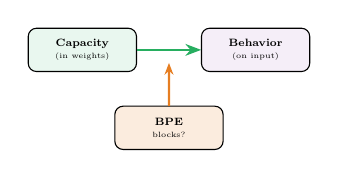
\begin{tikzpicture}[
  scale=0.55, transform shape,
  box/.style={draw, rounded corners=3pt, minimum height=1cm, minimum width=2.5cm,
              align=center, font=\scriptsize}
]
  \node[box, fill=circuit!10] (cap) at (0, 0) {\textbf{Capacity}\\{\tiny (in weights)}};
  \node[box, fill=fusion!10] (flow) at (4, 0) {\textbf{Behavior}\\{\tiny (on input)}};
  \node[box, fill=tok!15] (bpe) at (2, -1.8) {\textbf{BPE}\\{\tiny blocks?}};
  \draw[-{Stealth[length=2mm]}, thick, circuit] (cap) -- (flow);
  \draw[-{Stealth[length=1.5mm]}, thick, tok] (bpe) -- (2, -0.3);
\end{tikzpicture}
\end{center}
\end{minipage}

\vspace{0.5em}
\textbf{3. Novel-name generalization}
\begin{itemize}
  \item Test on names guaranteed absent from GPT-2's training data
  \item If the circuit generalizes, it's compositional computation --- not memorization
\end{itemize}
\end{frame}

% =============================================
% DISCUSSION: CAUSAL ABSTRACTION
% =============================================
\begin{frame}{Causal abstraction: what are we claiming? {\scriptsize(\href{https://arxiv.org/abs/2106.02997}{Geiger et al., 2021})}}
\hypertarget{sl:discussion}{}

\begin{columns}[c]
\begin{column}{0.42\textwidth}
\begin{center}
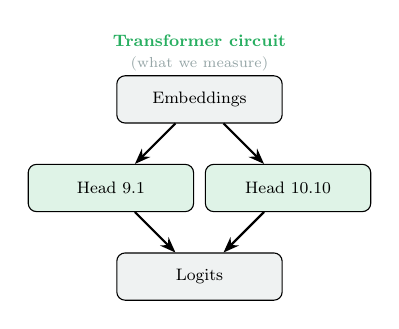
\begin{tikzpicture}[
  scale=0.75, transform shape,
  abox/.style={draw, rounded corners=3pt, minimum width=2.8cm, minimum height=0.8cm,
               align=center, font=\footnotesize},
  arr/.style={-{Stealth[length=2mm]}, thick},
]
  % Low-level transformer (LEFT)
  \node[abox, fill=chill!15] (emb) at (0, 4) {Embeddings};
  \node[abox, fill=circuit!15] (h1) at (-1.5, 2.5) {Head 9.1};
  \node[abox, fill=circuit!15] (h2) at (1.5, 2.5) {Head 10.10};
  \node[abox, fill=chill!15] (logit) at (0, 1) {Logits};

  \draw[arr] (emb) -- (h1);
  \draw[arr] (emb) -- (h2);
  \draw[arr] (h1) -- (logit);
  \draw[arr] (h2) -- (logit);

  \node[font=\footnotesize\bfseries, circuit] at (0, 5) {Transformer circuit};
  \node[font=\scriptsize, chill] at (0, 4.6) {(what we measure)};
\end{tikzpicture}
\end{center}
\end{column}

\begin{column}{0.16\textwidth}
\begin{center}
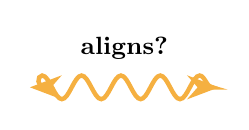
\begin{tikzpicture}
  \draw[{Stealth[length=4mm]}-{Stealth[length=4mm]}, ultra thick, backbone!80, decorate,
        decoration={snake, amplitude=1.5mm, segment length=5mm}]
        (-1.2, 0) -- (1.2, 0);
  \node[font=\small\bfseries] at (0, 0.5) {aligns?};
\end{tikzpicture}
\end{center}
\end{column}

\begin{column}{0.42\textwidth}
\begin{center}
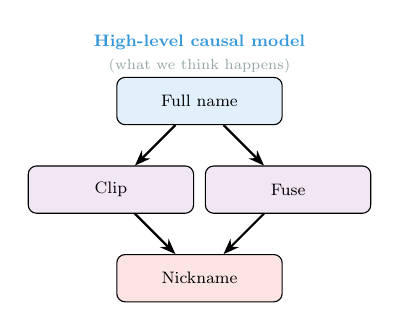
\begin{tikzpicture}[
  scale=0.75, transform shape,
  abox/.style={draw, rounded corners=3pt, minimum width=2.8cm, minimum height=0.8cm,
               align=center, font=\footnotesize},
  arr/.style={-{Stealth[length=2mm]}, thick},
]
  % High-level causal model (RIGHT)
  \node[abox, fill=accent!15] (name) at (0, 4) {Full name};
  \node[abox, fill=fusion!15] (clip) at (-1.5, 2.5) {Clip};
  \node[abox, fill=fusion!15] (fuse) at (1.5, 2.5) {Fuse};
  \node[abox, fill=phoneme!15] (out) at (0, 1) {Nickname};

  \draw[arr] (name) -- (clip);
  \draw[arr] (name) -- (fuse);
  \draw[arr] (clip) -- (out);
  \draw[arr] (fuse) -- (out);

  \node[font=\footnotesize\bfseries, accent] at (0, 5) {High-level causal model};
  \node[font=\scriptsize, chill] at (0, 4.6) {(what we think happens)};
\end{tikzpicture}
\end{center}
\end{column}
\end{columns}

\vspace{0.5em}
\textbf{IOI:} we \emph{expect} GPT-2 to track indirect objects --- the alignment is unsurprising.\\[3pt]
\textbf{Phonology:} GPT-2 was trained on text, never heard speech. If the alignment holds, this is a \emph{surprising generalization} --- phonological computation emerged from orthographic co-occurrence data alone.
\end{frame}

% =============================================
\begin{frame}{What is a ``mechanism''? Our hypothesis}
\hypertarget{sl:mechanism}{}

\begin{center}
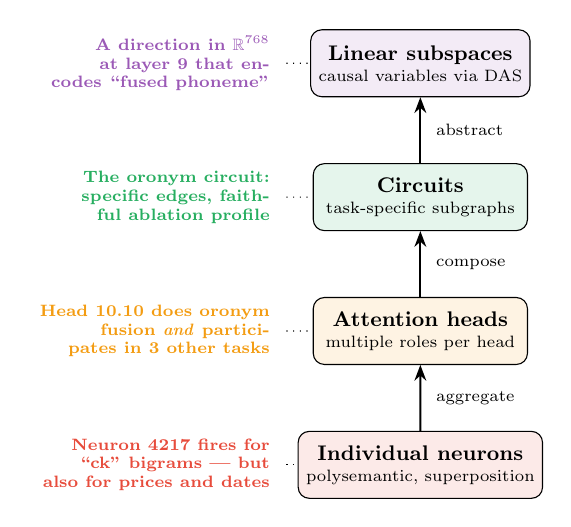
\begin{tikzpicture}[
  scale=0.85, transform shape,
  level/.style={draw, rounded corners=4pt, minimum width=3.2cm, minimum height=1cm,
                align=center, font=\small},
  arr/.style={-{Stealth[length=2mm]}, thick, black},
]
  % Levels of description
  \node[level, fill=phoneme!12] (neuron) at (0, 0) {
    \textbf{Individual neurons}\\[-2pt]
    {\scriptsize polysemantic, superposition}
  };
  \node[level, fill=backbone!12] (head) at (0, 2) {
    \textbf{Attention heads}\\[-2pt]
    {\scriptsize multiple roles per head}
  };
  \node[level, fill=circuit!12] (circuit) at (0, 4) {
    \textbf{Circuits}\\[-2pt]
    {\scriptsize task-specific subgraphs}
  };
  \node[level, fill=fusion!12] (subspace) at (0, 6) {
    \textbf{Linear subspaces}\\[-2pt]
    {\scriptsize causal variables via DAS}
  };

  \draw[arr] (neuron) -- (head) node[midway, right, font=\scriptsize, xshift=3pt, black] {aggregate};
  \draw[arr] (head) -- (circuit) node[midway, right, font=\scriptsize, xshift=3pt, black] {compose};
  \draw[arr] (circuit) -- (subspace) node[midway, right, font=\scriptsize, xshift=3pt, black] {abstract};

  % Annotations on left
  \node[font=\scriptsize\bfseries, text width=3.5cm, align=right, phoneme] at (-4, 0) {
    Neuron 4217 fires for ``ck'' bigrams --- but also for prices and dates
  };
  \node[font=\scriptsize\bfseries, text width=3.5cm, align=right, backbone] at (-4, 2) {
    Head 10.10 does oronym fusion \emph{and} participates in 3 other tasks
  };
  \node[font=\scriptsize\bfseries, text width=3.5cm, align=right, circuit] at (-4, 4) {
    The oronym circuit: specific edges, faithful ablation profile
  };
  \node[font=\scriptsize\bfseries, text width=3.5cm, align=right, fusion] at (-4, 6) {
    A direction in $\mathbb{R}^{768}$ at layer 9 that encodes ``fused phoneme''
  };

  \draw[dotted, black] (-2, 0) -- (neuron.west);
  \draw[dotted, black] (-2, 2) -- (head.west);
  \draw[dotted, black] (-2, 4) -- (circuit.west);
  \draw[dotted, black] (-2, 6) -- (subspace.west);

\end{tikzpicture}
\end{center}

\vspace{0.3em}
No single level is ``the mechanism.'' Each level answers a different question ---
and each has known failure modes (superposition, polysemanticity, multiple roles).
\end{frame}

% =============================================
\begin{frame}{The cognitive science parallel}
\hypertarget{sl:cogsci}{}

\begin{columns}[T]
\begin{column}{0.5\textwidth}
\textbf{Double dissociation} (Shallice, 1988):
\begin{itemize}
  \item Lesion region A $\Rightarrow$ lose ability X, keep Y
  \item Lesion region B $\Rightarrow$ keep X, lose Y
  \item Strong evidence for modularity
\end{itemize}

\vspace{0.5em}
\textbf{What we find:}
\begin{itemize}
  \item Ablate head 10.10 $\Rightarrow$ oronym breaks, hypocorism survives
  \item Ablate head 9.1 $\Rightarrow$ hypocorism breaks, oronym survives
  \item \textcolor{circuit}{Double dissociation across 6 tasks}
\end{itemize}
\end{column}

\begin{column}{0.5\textwidth}
\textbf{But dissociation $\neq$ understanding:}
\begin{itemize}
  \item A calculator dissociates $+$ from $\times$ --- nobody calls that ``understanding addition''
  \item The question: is phonological assembly \emph{compositional computation} or \emph{lookup}?
  \item Novel names (unseen in training) are the critical test
\end{itemize}

\vspace{0.5em}
\textbf{What would change our mind:}
\begin{itemize}
  \item[\textcolor{circuit}{$\checkmark$}] Clean dissociations {\scriptsize (have this)}
  \item[\textcolor{circuit}{$\checkmark$}] Faithful circuits {\scriptsize (have this)}
  \item[\textcolor{backbone}{?}] DAS subspaces {\scriptsize (running)}
  \item[\textcolor{phoneme}{$\times$}] Novel-name generalization {\scriptsize (future)}
\end{itemize}
\end{column}
\end{columns}

\end{frame}

% =============================================
\begin{frame}{Limitation 1: circuits are a wiring diagram, not a content map}
\hypertarget{sl:tooling}{}

\begin{center}
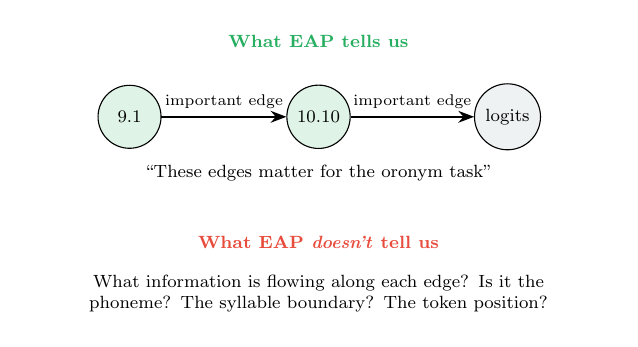
\begin{tikzpicture}[
  scale=0.8, transform shape,
  nd/.style={draw, circle, minimum size=1cm, align=center, font=\footnotesize},
  arr/.style={-{Stealth[length=2mm]}, thick},
]
  % What we get
  \node[nd, fill=circuit!15] (a) at (0, 0) {9.1};
  \node[nd, fill=circuit!15] (b) at (3, 0) {10.10};
  \node[nd, fill=chill!15] (c) at (6, 0) {logits};
  \draw[arr] (a) -- (b) node[midway, above, font=\scriptsize] {important edge};
  \draw[arr] (b) -- (c) node[midway, above, font=\scriptsize] {important edge};

  \node[font=\footnotesize\bfseries, circuit] at (3, 1.2) {What EAP tells us};
  \node[font=\footnotesize, black] at (3, -0.9) {``These edges matter for the oronym task''};

  % What we don't get
  \node[font=\footnotesize\bfseries, phoneme] at (3, -2) {What EAP \emph{doesn't} tell us};
  \node[font=\footnotesize, black, text width=9cm, align=center] at (3, -2.8) {
    What information is flowing along each edge?
    Is it the phoneme? The syllable boundary? The token position?
  };
\end{tikzpicture}
\end{center}

\vspace{0.3em}
\begin{itemize}
  \item EAP and activation patching find \emph{which} heads matter --- not \emph{what} they compute
  \item A single head can serve multiple roles across tasks (head 10.10 appears in 4 circuits)
  \item We need methods that decompose \emph{within} an edge: what subspace of the residual stream carries the phonological signal from one head to the next?
\end{itemize}
\end{frame}

% =============================================
\begin{frame}{Limitation 2: the nonlinear representation dilemma}

\textbf{The dilemma} (\href{https://arxiv.org/abs/2507.08802}{Sutter et al., NeurIPS 2025}):

\vspace{0.3em}
\begin{columns}[T]
\begin{column}{0.48\textwidth}
With \emph{unrestricted} nonlinear alignment maps:
\begin{itemize}
  \item \textbf{Any} model maps to \textbf{any} algorithm
  \item Even \emph{randomly initialized} GPT-2 achieves 100\% IIA on IOI
  \item Causal abstraction becomes vacuous
\end{itemize}

\vspace{0.3em}
DAS avoids this by restricting to \emph{linear} maps --- but that might miss real nonlinear structure.
\end{column}

\begin{column}{0.48\textwidth}
\textbf{A possible way forward:}
\begin{itemize}
  \item Use \emph{restricted} nonlinear maps --- constrained enough to be informative, flexible enough to find curved representations
  \item The constraint is what gives causal abstraction its power --- the question is finding the right constraint
\end{itemize}

\vspace{0.3em}
If DAS finds high IIA with linear maps, that's meaningful \emph{because} we constrained ourselves. $\Rightarrow$ We are exploring restricted nonlinear maps in parallel work.
\end{column}
\end{columns}
\end{frame}

% =============================================
% FUTURE: CAUSAL GRAPH DISCOVERY FOR VARIABLES
% =============================================
\begin{frame}{Future: discovering the causal graph, not assuming it}

\textbf{Current approach:} We hypothesize a causal model (name $\to$ shorten $\to$ fuse $\to$ output) and test alignment via DAS.

\vspace{0.3em}
\textbf{The gap:} We test \emph{our} graph. What if the model implements a different causal structure?

\vspace{0.5em}
\textbf{Proposed experiment:}
\begin{enumerate}
  \item Use PC/CD-NOD on \textbf{DAS-learned causal variables} (not raw head activations) to discover the DAG connecting phonological operations
  \item For chained operations (oronyms), test whether the discovered graph is name $\to$ shorten $\to$ fuse $\to$ output vs.\ name $\to$ output directly
  \item Compare discovered DAGs between simple tasks (hypocorism: 1 step) and compound tasks (oronym: 2+ steps)
\end{enumerate}

\vspace{0.3em}
{\small This combines our circuit validation (causal discovery finds the same heads) with causal variable localization (DAS finds what flows) --- applying causal inference at the \emph{variable} level rather than the \emph{head} level.}
\end{frame}

% =============================================
% STATUS
% =============================================
\begin{frame}{Current status}

\begin{center}
\small
\begin{tabular}{lll}
\toprule
\textbf{Component} & \textbf{Status} & \textbf{Next step} \\
\midrule
Paper outline & \textcolor{circuit}{Complete} & --- \\
6 operation definitions & \textcolor{circuit}{Complete} & --- \\
Minimal-pair datasets & \textcolor{circuit}{Complete} & 446 pairs across 6 ops \\
Behavioral validation & \textcolor{circuit}{Complete} & All 6 ops $>$70\% accuracy \\
EAP-IG circuit discovery & \textcolor{circuit}{Complete} & All circuits faithful \\
\midrule
Activation patching & \textcolor{circuit}{Complete} & Validates EAP head rankings \\
Causal discovery & \textcolor{circuit}{Complete} & PC + CD-NOD on head activations \\
DAS probing & \textcolor{circuit}{Complete} & Rank-1 causal subspaces per layer \\
Circuit overlap analysis & \textcolor{circuit}{Complete} & Backbone + specialist structure \\
\midrule
Compositional ablation & \textcolor{backbone}{Next} & Ablate sub-circuits in chained ops \\
Tokenization experiment & \textcolor{backbone}{Next} & Slash-condition test \\
Cross-task DAS transfer & \textcolor{backbone}{Next} & Do tasks share causal directions? \\
Causal graph discovery & \textcolor{backbone}{Next} & CD-NOD / LiNGAM on head activations \\
\bottomrule
\end{tabular}
\end{center}

\end{frame}

% =============================================
% THANK YOU
% =============================================
\begin{frame}{Thank you}

\begin{center}
\vfill
{\Large Phonological Assembly Circuits in GPT-2}

\vspace{1.5em}

\textbf{Repository:} \href{https://github.com/elliottower/phonetic-circuits}{\texttt{github.com/elliottower/phonetic-circuits}}

\textbf{Contact:} \texttt{elliot@elliottower.ai}

\vspace{1.5em}

\vfill
\end{center}
\end{frame}

\end{document}
